\documentclass[12pt]{article}
\usepackage[utf8]{inputenc}
\usepackage[spanish]{babel}
\usepackage{siunitx}
% ---------------------------------------------------
%                       FONT 
% ---------------------------------------------------

\usepackage{cmbright}                               % Font
\documentclass{article}
\usepackage{siunitx}
\usepackage{hyperref} % LINKS
\usepackage{caption}
\decimalpoint
\usepackage{mathtools}
\usepackage{amsmath}
\usepackage{amsthm}
\usepackage{amssymb}
\usepackage{graphicx}
\usepackage[margin=0.9in]{geometry}
\usepackage{fancyhdr}
\usepackage[inline]{enumitem}
\usepackage{float}
\usepackage{cancel}
\usepackage{bigints}
\usepackage{color}
\usepackage{xcolor}
\usepackage{listingsutf8}
\usepackage{algorithm}
\usepackage{tocloft}
\usepackage[none]{hyphenat}
\usepackage{graphicx}
\usepackage{grffile}
\usepackage{tabularx}
\usepackage[nottoc,notlot,notlof]{tocbibind}
\usepackage{times}
\usepackage{color}
\usepackage{enumitem}
\usepackage{amsfonts}
\definecolor{gray97}{gray}{.97}
\definecolor{gray75}{gray}{.75}
\definecolor{gray45}{gray}{.45}
\renewcommand{\cftsecleader}{\cftdotfill{\cftdotsep}}
\pagestyle{fancy}
\setlength{\headheight}{15pt} 
\lhead{Práctica 5: Fotopletismógrafo}
\rhead{\thepage}
\lfoot{ESCOM-IPN}
\renewcommand{\footrulewidth}{0.5pt}
\setlength{\parskip}{0.5em}
\newcommand{\ve}[1]{\overrightarrow{#1}}
\newcommand{\abs}[1]{\left\lvert #1 \right\lvert}
\date{ 01 de Junio 2018}
\title{Amplificador}
\author{Instrumentacion}
\usepackage[
  separate-uncertainty = true,
  multi-part-units = repeat
]{siunitx}

\definecolor{pblue}{rgb}{0.13,0.13,1}
\definecolor{pgreen}{rgb}{0,0.5,0}
\definecolor{pred}{rgb}{0.9,0,0}
\definecolor{pgrey}{rgb}{0.46,0.45,0.48}
\lstset{tabsize=1}
\usepackage{wrapfig}
\usepackage{multicol}
\usepackage{listings}
\lstset{ frame=Ltb,
framerule=0pt,
aboveskip=0.5cm,
framextopmargin=3pt,
framexbottommargin=3pt,
framexleftmargin=0.4cm,
framesep=0pt,
rulesep=.4pt,
backgroundcolor=\color{gray97},
rulesepcolor=\color{black},
%
stringstyle=\ttfamily,
showstringspaces = false,
basicstyle=\small\ttfamily,
commentstyle=\color{gray45},
keywordstyle=\bfseries,
%
numbers=left,
numbersep=15pt,
numberstyle=\tiny,
numberfirstline = false,
breaklines=true,
}

% minimizar fragmentado de listados
\lstnewenvironment{listing}[1][]
{\lstset{#1}\pagebreak[0]}{\pagebreak[0]}

\lstdefinestyle{consola}
{basicstyle=\scriptsize\bf\ttfamily,
backgroundcolor=\color{gray75},
}

\lstdefinestyle{Java}
{language=Java,
}

%%%%%%%%%%%%%%%%%%%%%

\lstdefinestyle{customc}{
  belowcaptionskip=1\baselineskip,
  breaklines=true,
  frame=L,
  xleftmargin=\parindent,
  language=C,
  showstringspaces=false,
  basicstyle=\footnotesize\ttfamily,
  keywordstyle=\bfseries\color{green!40!black},
  commentstyle=\itshape\color{purple!40!black},
  identifierstyle=\color{blue},
  stringstyle=\color{orange},
}

\lstdefinestyle{customasm}{
  belowcaptionskip=1\baselineskip,
  frame=L,
  xleftmargin=\parindent,
  language=[x86masm]Assembler,
  basicstyle=\footnotesize\ttfamily,
  commentstyle=\itshape\color{purple!40!black},
}

\lstset{escapechar=@,style=customc}

% Ayuda para el formato de las tablas
\usepackage{array}
% Se declara un nuevo tipo de columna para alinear de manera:
% -Horizontal
\newcolumntype{P}[1]{>{\centering\arraybackslash}p{#1}}
% -Vertical
\newcolumntype{M}[1]{>{\centering\arraybackslash}m{#1}}

% Indica la separacion entre las columnas de una tabla
\setlength{\tabcolsep}{10pt} % Default value: 6pt
% Indica el padding inferior y superior de las celdas de una tabla
\renewcommand{\arraystretch}{1.8} % Default value: 1

\usepackage{longtable}
%Permite crear columnas en el documento
\usepackage{multicol}
\usepackage{color}
\usepackage{comment}
\newcommand{\tabitem}{~~\llap{\textbullet}~~}
\newcommand{\subtabitem}{~~~~\llap{\textbullet}~~}

\bibliographystyle{IEEEtran}
\begin{document}
        \begin{titlepage}
            \begin{center}
                
                % Upper part of the page. The '~' is needed because \\
                % only works if a paragraph has started.
                
                \noindent
                \begin{minipage}{0.5\textwidth}
                    \begin{flushleft} \large
                        \includegraphics[width=0.5\textwidth]{../ipn.png}
                    \end{flushleft}
                \end{minipage}%
                \begin{minipage}{0.55\textwidth}
                    \begin{flushright} \large
                        \includegraphics[width=0.4\textwidth]{../escom.png}
                    \end{flushright}
                \end{minipage}
                
                \textsc{\LARGE Instituto Politécnico Nacional}\\[0.5cm]
                
                \textsc{\Large Escuela Superior de Cómputo}\\[1cm]
                
                % Title
                
                { \huge Práctica 5: Fotopletismógrafo \\[1cm] }
                
                { \Large Unidad de aprendizaje: Instrumentación} \\[1cm]
                
                { \Large Grupo: 3CM4 } \\[1cm]
                
                \noindent
                \begin{minipage}{0.5\textwidth}
                    \begin{flushleft} \large
                        \emph{Integrantes:}\\
                        
                        \begin{tabular}{ll}
                        Aguilar Herrera Arianna Itzamina \\
                        Nicolás Sayago Abigail\\
                        Ramos Diaz Enrique \\
                    \end{tabular}
                    \end{flushleft}
                \end{minipage}%
                \begin{minipage}{0.5\textwidth}
                    \begin{flushright} \large
                        \emph{Profesor(a):} \\
                        Tellez Barrera Juan Carlos  \\
                    \end{flushright}
                \end{minipage}
                
                \vfill
                
                % Bottom of the page
                {\large Fecha de entrega: 28 de octubre de 2018}
            \end{center}
        \end{titlepage}
    
    \tableofcontents
    \newpage
    
    % /////////////////////////////////////////////////////////////////////
    %                           OBJETIVOS
    % ////////////////////////////////////////////////////////////////////
    \section{Objetivo}
        \begin{itemize}
            \item[\checkmark] Aprender el uso y características del sensor de reflexión infrarrojo TCRT5000L
             \item[\checkmark] Graficar los pulsos del corazón con ayuda de un instrumento, el fotopletismógrafo. 
             \item[\checkmark] Interpretar y leer señales producidas por el pulso cardíaco.
             \item[\checkmark] Repasar el funcionamiento del amplificador operacional derivador y el amplificador operacional integrador.
        \end{itemize}
    
    
        % /////////////////////////////////////////////////////////////////////
    %                           EQUIPO
    % ////////////////////////////////////////////////////////////////////
    \section{Listado de materiales}
        
        \begin{multicols}{2}
        
            \textbf{Resistores:}
            \begin{itemize}
                \item 1 de 150 $\Omega$
                \item 3 de 1 $k\Omega$
                \item 2 de 10 $k\Omega$
                \item 2 de 220 $k\Omega$
                \item 3 de 330 $k\Omega$
            \end{itemize}
            
            \textbf{Preset ó Potenciometro:}
            \begin{itemize}
                \item 1 de 10 $k\Omega$
            \end{itemize}
            
            \textbf{Capacitores:}
            \begin{itemize}
                \item 5 de $.47$ microF o $470$ nanoF
                \item 1 de 100 $nF$
            \end{itemize}

      \columnbreak
    
          \textbf{Semiconductores:}
            \begin{itemize}
                \item 1 Sensor de reflexión infrarrojo TCRT5000L
                \item 1 Diodo LED
            \end{itemize}

        \textbf{Circuitos integrados:}
            \begin{itemize}
                \item 1 LM741 OPAMP  (alimentación $\pm12V$)
            \end{itemize}   
            
        \textbf{Opcionales:}
            \begin{itemize}
                \item 1 Transistor BC547
                \item 1 Resistor 1$K\Omega$
            \end{itemize}
      
      \end{multicols}
      
    \section{Listado de equipo}
      
        \begin{itemize}
            \item 1 Voltímetro digital.
            \item 1 Fuente de alimentación.
            \item 1 Osciloscopio digital
        \end{itemize}
        
    
    % /////////////////////////////////////////////////////////////////////
    %                           INTRODUCCION
    % ////////////////////////////////////////////////////////////////////

    \section{Introducción}
        \subsection{Flotopletismografía}
            Un pletismógrafo es un dispositivo que mide la cantidad de sangre en una parte del cuerpo. Un fotopletismógrafo hace esto ópticamente. 
            
            Es una técnica de pletismografía, es decir, medición de cambios de presión y volumen que se utiliza para medir parámetros orientados al diagnóstico de enfermedades pulmonares o cardiovasculares en la cual se utiliza un haz de luz para determinar el volumen de un órgano.
            
            Se utiliza principalmente en:
            \begin{itemize}
                \item Ciclo cardíaco 
                \item Flujo sanguíneo
                \item Respiración
                \item Efectividad en la anestesia
            \end{itemize}
            
            Se basa en un principio: \textbf{se aproxima el volumen de un cuerpo determinando la cantidad de luz que este refleja}.
            
            \begin{figure}[h!]
                \centering
                \includegraphics[width=0.6\textwidth]{Practica5/Images/foto3.jpg}
            \end{figure}
            
        \subsection{Funcionamiento}
        En teoría, el fotopletismógrafo es simple: mide la variación en la cantidad de luz que pasa a través de su dedo causada por la naturaleza pulsátil del flujo sanguíneo.
        
        \begin{figure}[h!]
                \centering
                \includegraphics[width=\textwidth]{Practica5/Images/foto.PNG}
            \end{figure}
        
        Un fuente de luz infrarroja (LED) emite un haz sobre la piel para iluminar los vasos subcutáneos, estos reflejan parte de dicho haz dependiendo la cantidad de hematíes que contienen. La luz reflejada incide en un fotosensor (usualmente de cadmio-selenio) que la convierte en un voltaje equivalente. 
        
        Debido a que la piel absorbe más del  $90\%$ de la luz, el par diodo-fotosensor se acompaña de amplificadores y filtros que garantizan un voltaje adecuado. El ciclo cardíaco puede obtenerse midiendo el intervalo que existe entre cada pico de voltaje.
            
        La calidad de las mediciones realizadas utilizando esta técnica dependen de la ubicación del emisor y receptor de luz, las características de los tejidos de cada paciente, la calidad de los amplificadores y filtros, entre otros. No obstante, su uso es generalizado teniendo en cuenta su bajo costo y su carácter no invasivo
        
        La señal que se trata de observar consiste en variaciones muy pequeñas (cambios en la intensidad de la luz debidos al flujo de sangre hacia o desde el dedo), superpuestas a una señal constante grande (luz promedio que fluye a través del dedo).  
        
        Es solo la parte de la señal que varía con el tiempo la que se debe amplificar. Para deshacerse de la señal de CC se puede utilizar un filtro de pasa altas.   
        
        Para asegurarse de que la señal de interés (el fotopletismógrafo) no sea eliminada por el filtro, la frecuencia de corte del filtro debe ser inferior a aproximadamente 1 Hz (una frecuencia cardíaca típica).
        
        \subsection{Amplificador operacional derivador}
        Un derivador es un circuito en el que la señal de salida es proporcional a la derivada en el tiempo de la señal de entrada. En otras palabras: La salida es proporcional a la velocidad de variación de la señal de la entrada.
        
        Cuando la señal de entrada es sinusoidal, la salida del derivador es como se muestra en el siguiente gráfico.
        
        \begin{figure}[h!]
                \centering
                \subfloat{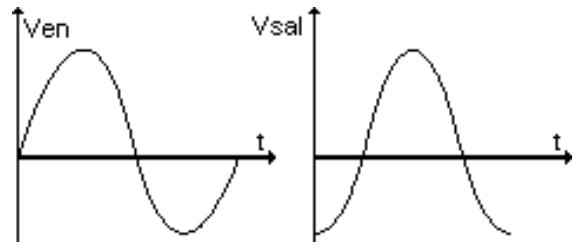
\includegraphics[width=0.5\textwidth]{Practica5/Images/der1.PNG}}
               \subfloat{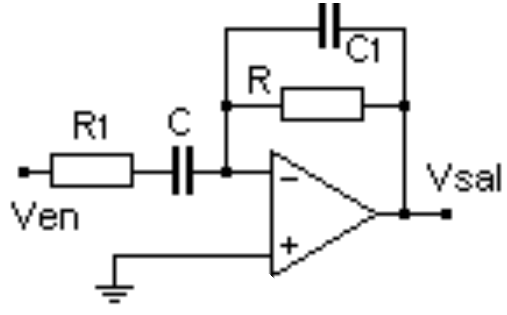
\includegraphics[width=0.4\textwidth]{Practica5/Images/der2.PNG}}
            \end{figure}
            
        \subsection{Amplificador operacional integrador}
        Un circuito integrador realiza un proceso de suma llamado “integración”. La tensión de salida del circuito integrador es proporcional al área bajo la curva de entrada (onda de entrada), para cualquier instante.
        
        En el primer gráfico (izquierda) se puede ver una señal de entrada (línea recta) de 3 voltios que se mantiene continuo con el pasar del tiempo. En el segundo gráfico (derecha) se muestra que el área bajo la curva en un momento cualquiera es igual al valor de la entrada multiplicado por el tiempo. 
        
        \begin{figure}[h!]
                \centering
                \subfloat{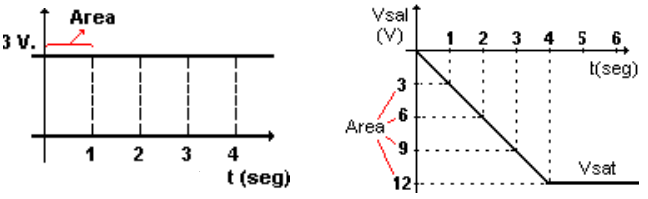
\includegraphics[width=0.5\textwidth]{Practica5/Images/int1.PNG}}
               \subfloat{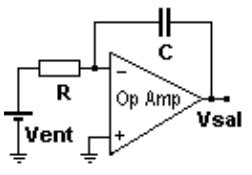
\includegraphics[width=0.4\textwidth]{Practica5/Images/int2.PNG}}
            \end{figure}



    % /////////////////////////////////////////////////////////////////////
    %                           DESARROLLO
    % ////////////////////////////////////////////////////////////////////
    \newpage
    \section{Desarrollo práctico}
        
        \subsection{PE 1 - Lectura de señal y Filtrado}
            \begin{multicols}{2}
                \subsubsection{Esquema}
                    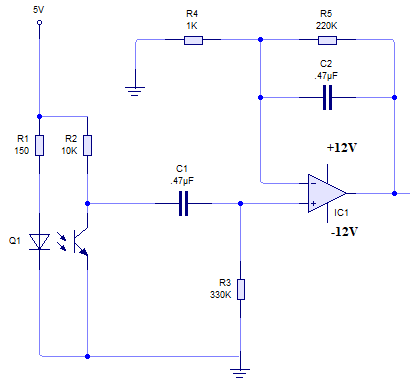
\includegraphics[width=0.5\textwidth]{Practica5/Images/pe1.png}
            
            \columnbreak
            
                \subsubsection{Circuito cableado}
                    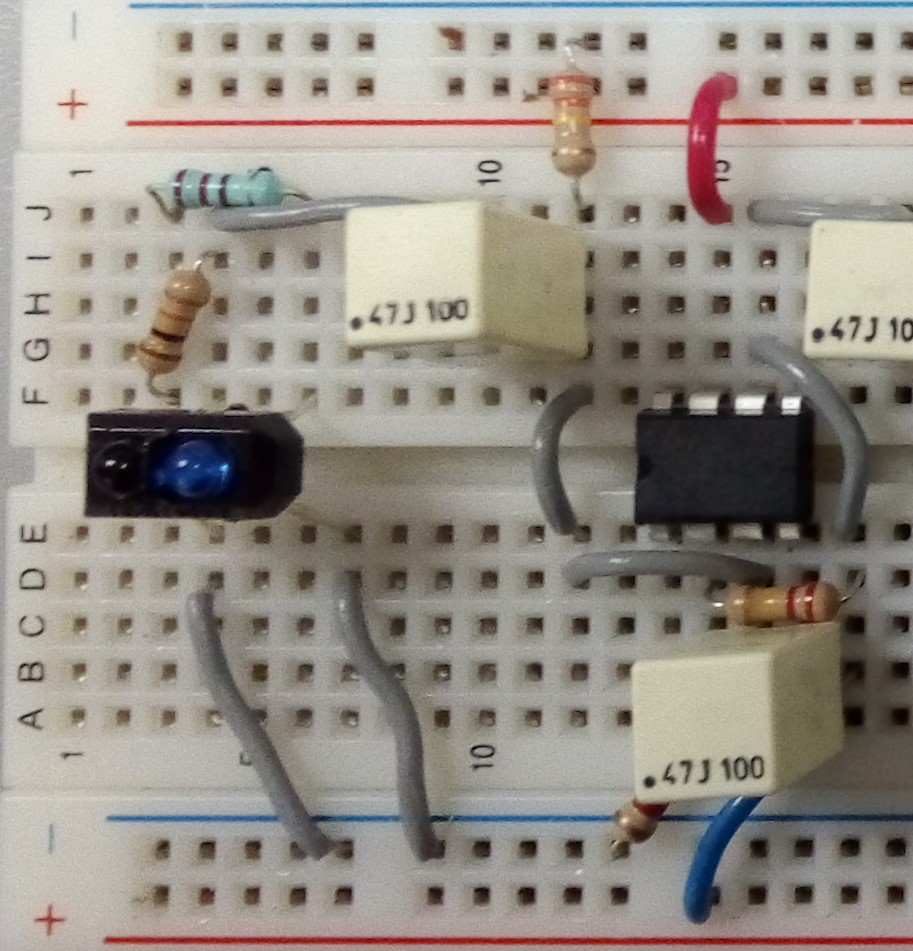
\includegraphics[width=0.4\textwidth]{Practica5/Images/cpe-1.jpg}
            \end{multicols}
            
            \subsubsection{Funcionamiento}
            Cuando colocamos el dedo encima del sensor TCRT5000L este leerá las pulsaciones de la persona como señales que consisten en variaciones muy pequeñas (cambios en la intensidad de la luz debido al flujo de sangre desde o hacia el dedo), la cual se mostrará en forma de señal en el osciloscopio. 
            
            Esta señal es sumamente pequeña y llena de ruido, por lo que pasa por varias etapas.
            
            \textbf{Etapa de amplificación y filtrado}     \\
            Una señal del pulso cardíaca ni siquiera alcanza los 100 mV, por lo que necesitamos amplificarla para su manejo. 
            
            Esta etapa posee dos capacitores y una configuración que también la hace funcionar como un filtro pasa bajas, que evita leer frecuencias extremadamente altas (ruido), proveniente de otras fuentes de luz y sombras, por ejemplo.
            
            Para probar el funcionamiento de esta etapa, conectamos la salida del LM741 al osciloscopio y colocamos nuestro dedo; también podemos pasar nuestra mano rápidamente por encima del sensor para que detecte los cambios de luz.
            
            Cada uno de los picos de voltaje equivale a un pulso cardíaco detectado (o cambio de luz).
            
             \textbf{Parámetros de medición (Vpp)}
            \begin{multicols}{2}
                \begin{itemize}
                    \item[\checkmark] \textbf{Amplitud máxima (Canal 2): 300 mV}
                    \item[\checkmark] \textbf{Base de tiempo: 500 ms}
            \columnbreak
                    \item[\checkmark] \textbf{Volts por división: 500 mV}
                    \item[\checkmark] \textbf{Acoplamiento: Corriente Alterna}
                \end{itemize}
            \end{multicols}
            
            \textbf{Nota:} La linea amarilla (Canal 1) es la señal que sale directamente del sensor y la azul (Canal 2) la que sale amplificada y filtrada.
         
            \begin{center}
            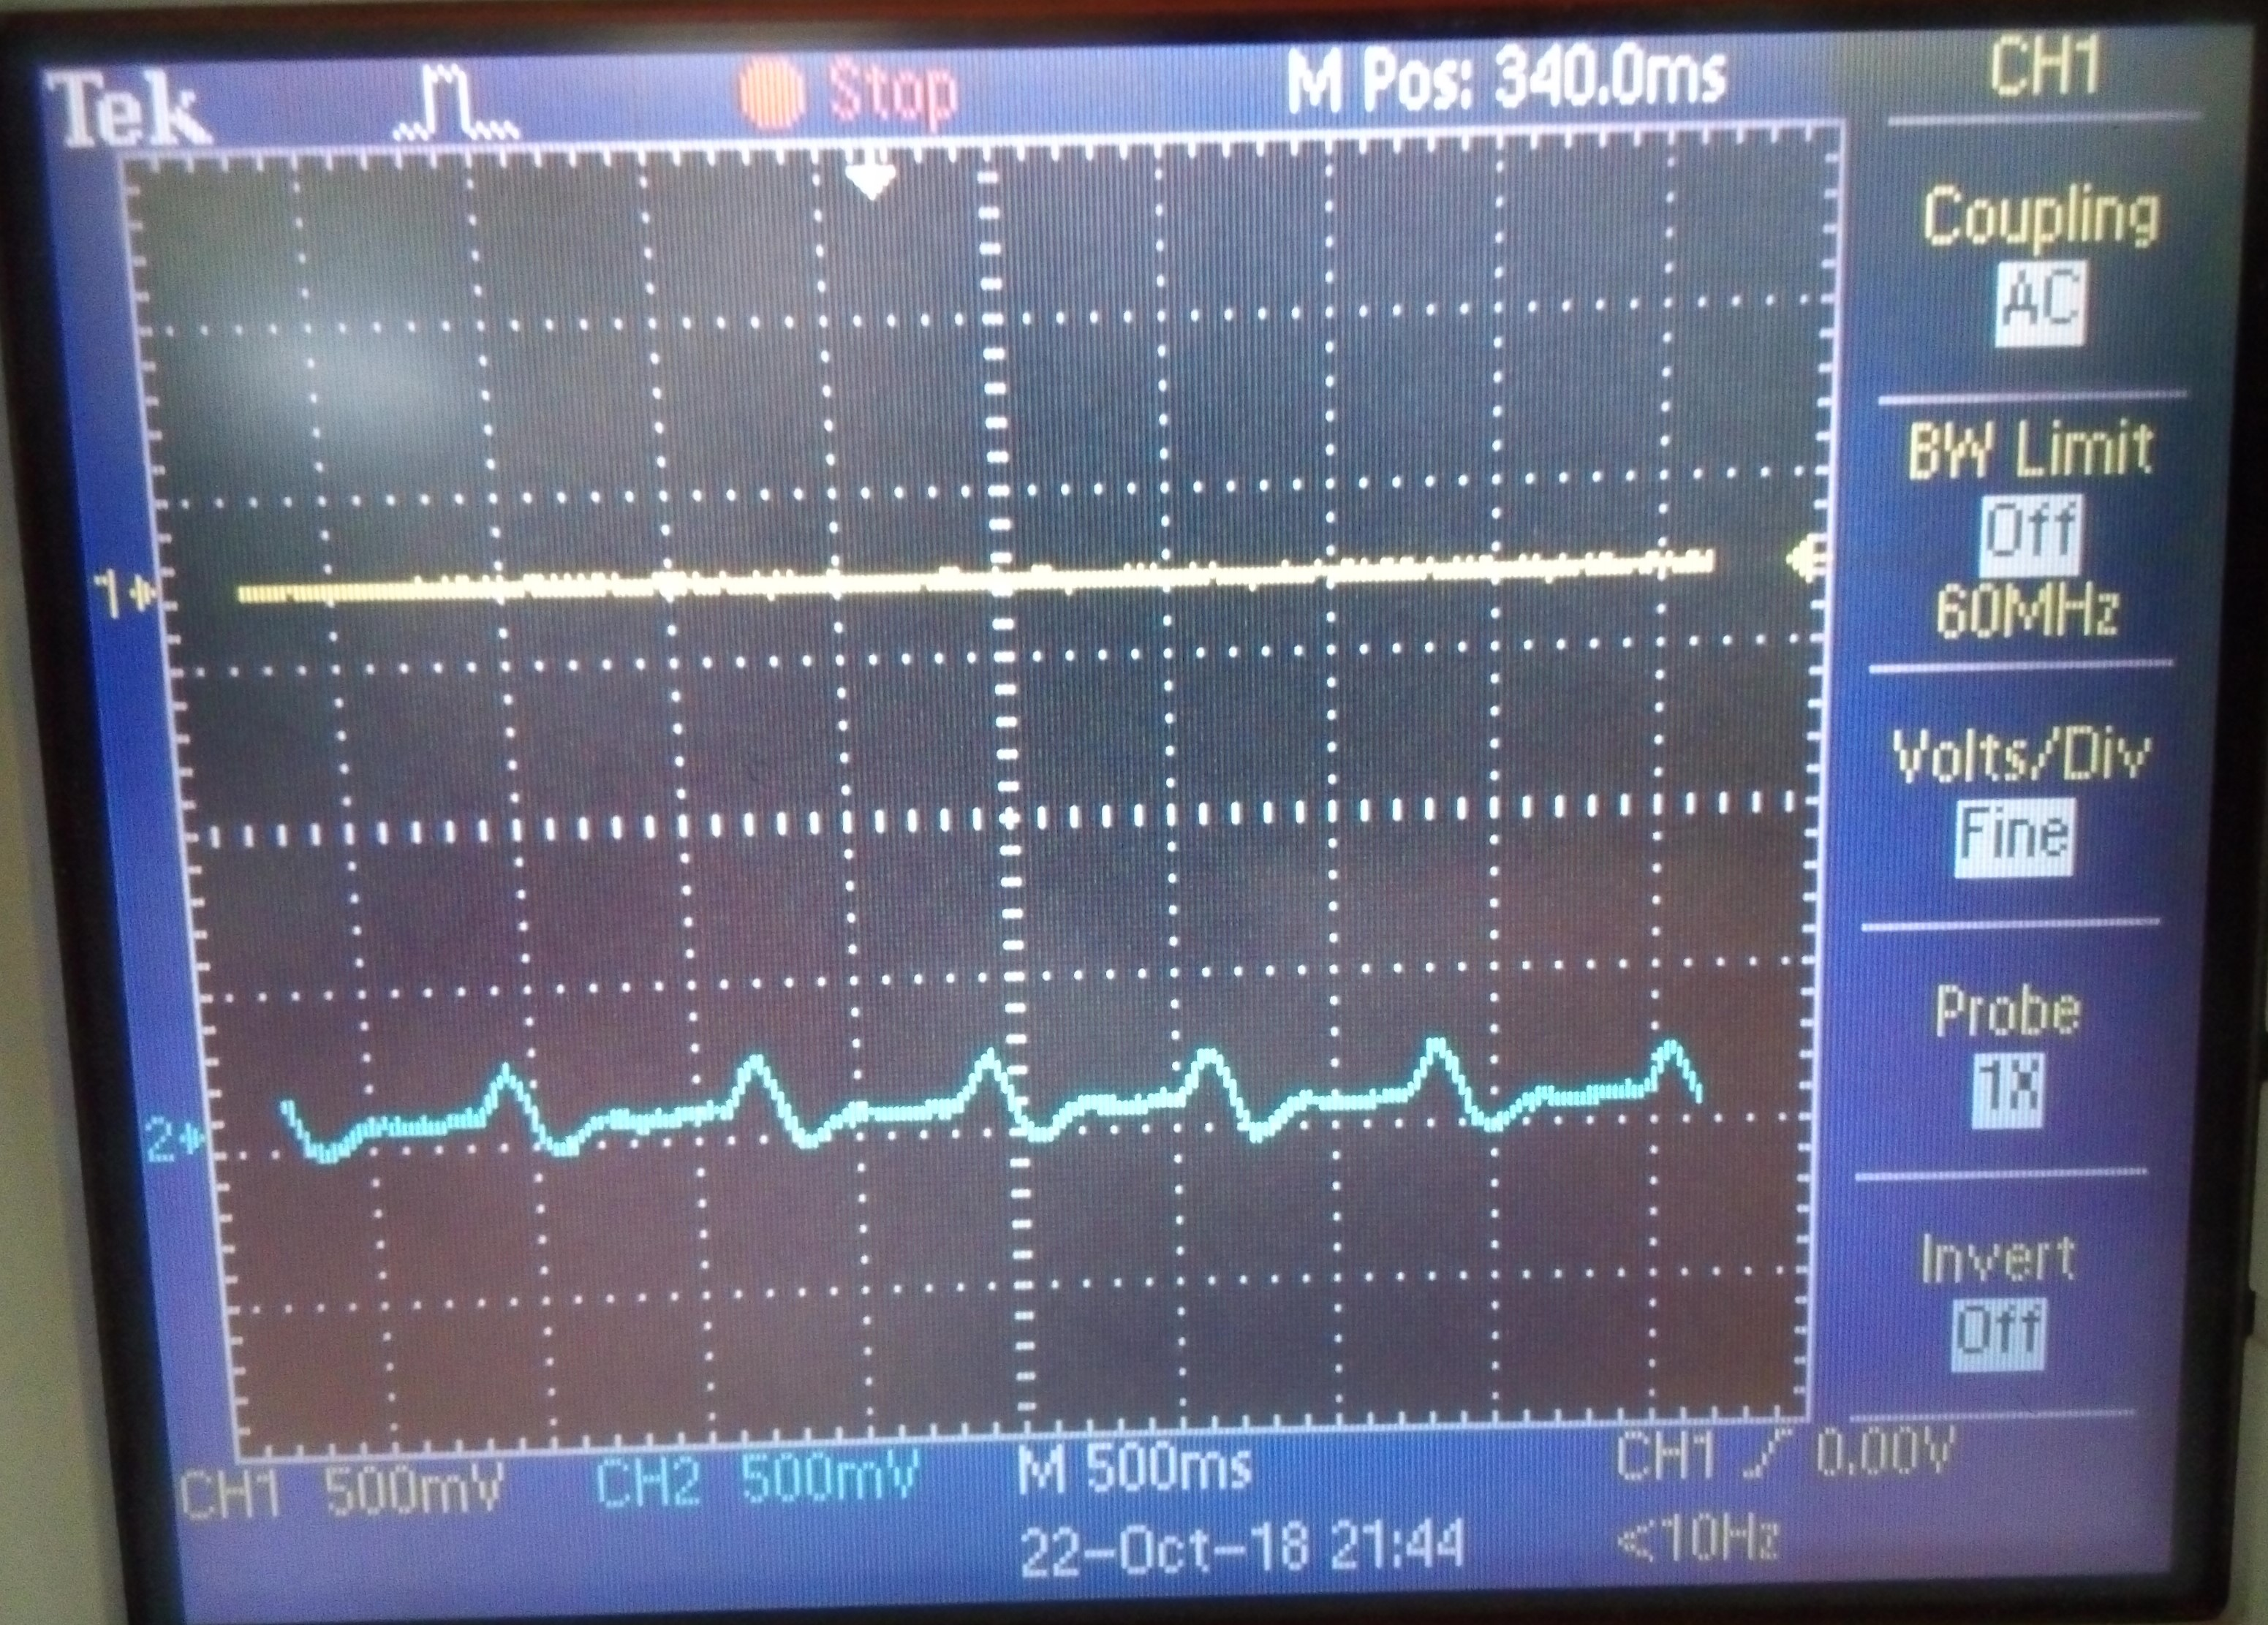
\includegraphics[width=0.65\textwidth]{Practica5/Images/etapa1_2.jpg}
            \end{center}
              
        \subsection{PE 2 - Derivador}
        \begin{multicols}{2}
            \subsubsection{Esquema}

                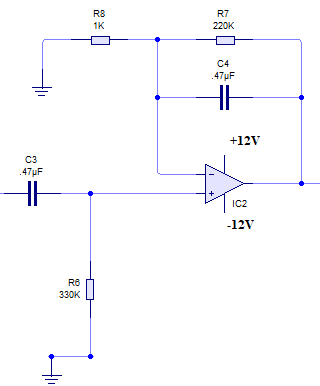
\includegraphics[width=0.38\textwidth]{Practica5/Images/pe2.png}

        \columnbreak
            \subsubsection{Circuito cableado}

                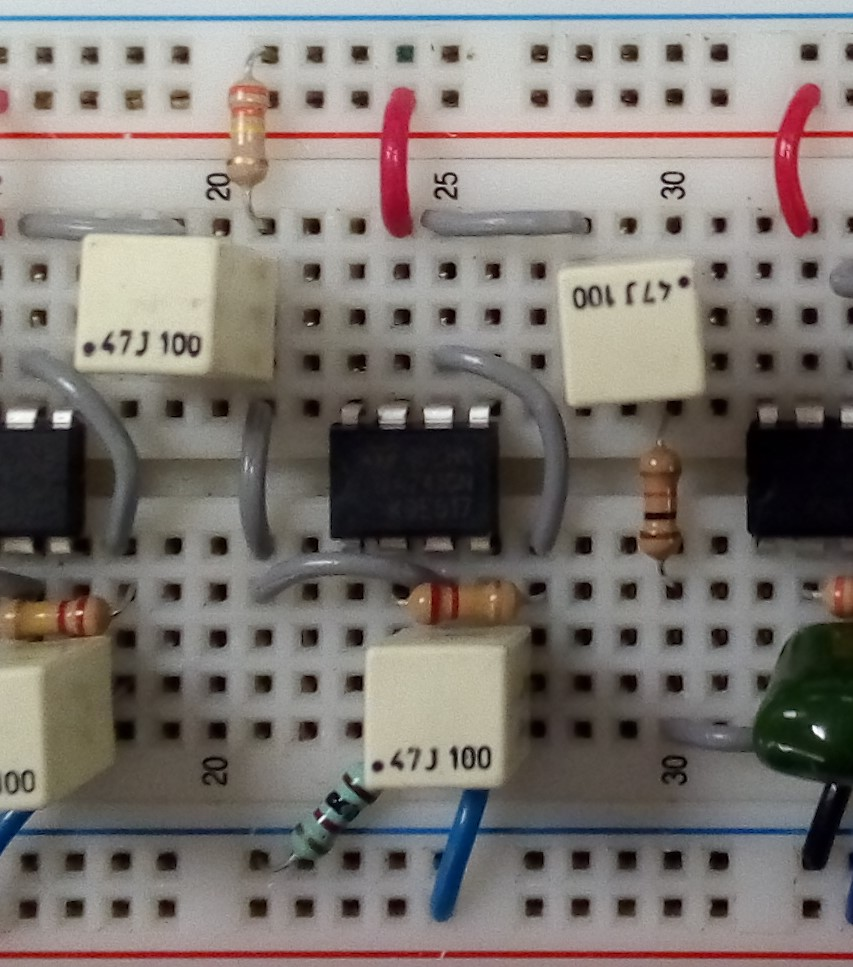
\includegraphics[width=0.4\textwidth]{Practica5/Images/cpe-2.jpg}

            \end{multicols}
            
        \subsubsection{Funcionamiento}
        
        Con el circuito derivador la señal de salida es proporcional a la derivada en el tiempo de la señal de entrada. En otras palabras: La salida es proporcional a la velocidad de variación de la señal de la entrada. Esto es de gran importancia para nuestro circuito puesto que estamos midiendo señales que cambian constantemente con el tiempo, y este tiempo es pequeño.

        \textbf{Parámetros de medición (Vpp)}
            \begin{multicols}{2}
                \begin{itemize}
                    \item[\checkmark] \textbf{Amplitud máxima (Canal 1): 8.4 V}
                
                    \item[\checkmark] \textbf{Amplitud máxima (Canal 2): 280 mV}
                    \item[\checkmark] \textbf{Base de tiempo: 500 ms}
            \columnbreak
                    \item[\checkmark] \textbf{Volts por división (CH1): 2 V}
                    \item[\checkmark] \textbf{Volts por división (CH2): 200 mV}
                    \item[\checkmark] \textbf{Acoplamiento: Corriente Alterna}
                \end{itemize}
            \end{multicols}
            
            \textbf{Nota:} La linea amarilla (Canal 1) es la señal que sale del derivador (Canal 2) la que sale filtrada y amplificada. 
         
            \begin{figure}[h!]
                \centering
                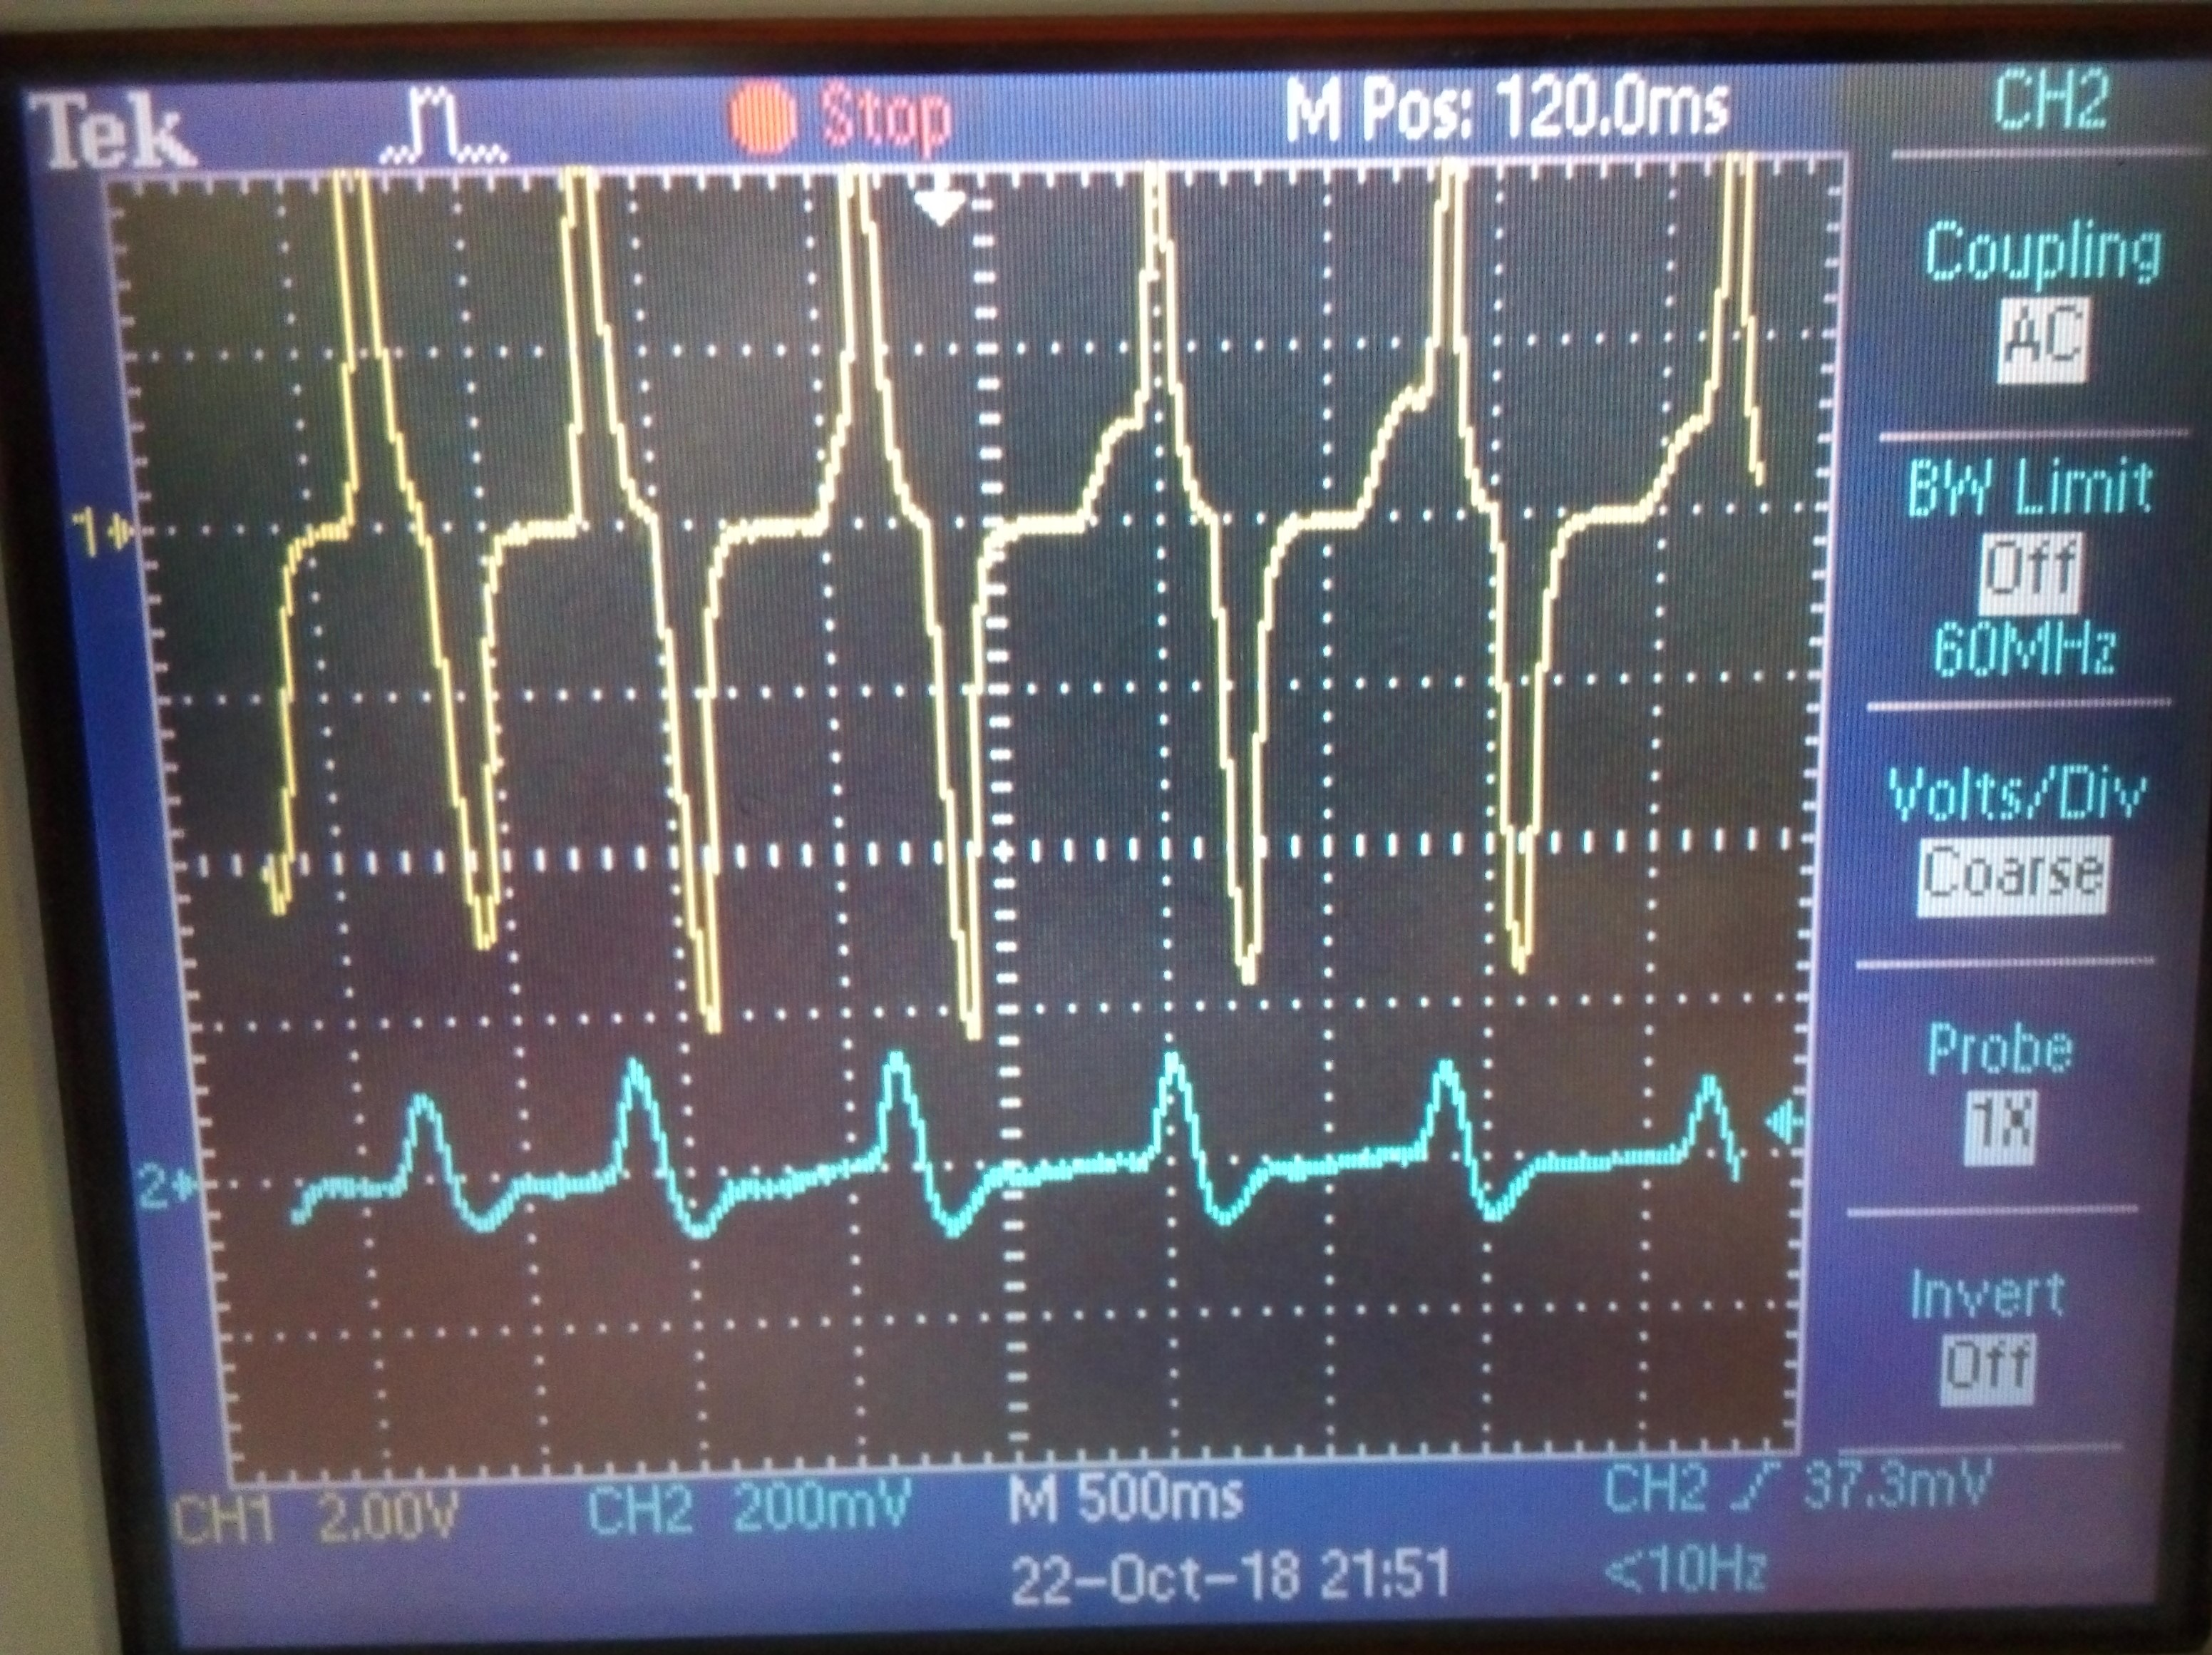
\includegraphics[width=0.65\textwidth]{Practica5/Images/etapa2_2.jpg}
            \end{figure}
        \newpage
        \subsection{PE 3 - Integrador}
        \begin{multicols}{2}
            \subsubsection{Esquema}

                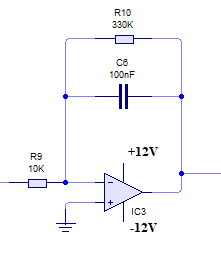
\includegraphics[width=0.45\textwidth]{Practica5/Images/pe3.png}

        \columnbreak
            \subsubsection{Circuito cableado}

                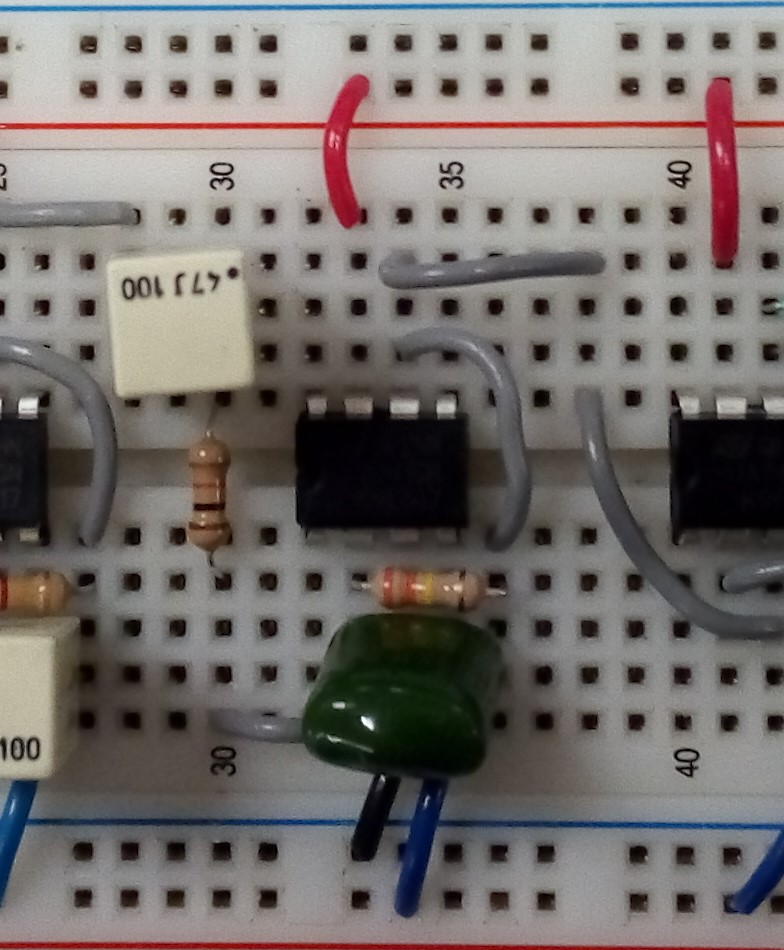
\includegraphics[width=0.4\textwidth]{Practica5/Images/cpe-3.jpg}

            \end{multicols}
            
            \subsubsection{Funcionamiento}
            
             %------------PONER FUNCIONAMIENTO Integrador (Integrar picos pequeños a los grandes)
             Hablando matemáticamente, un circuito integrador realiza un proceso de suma llamado \textsc{integración}. La tensión de salida del circuito integrador es proporcional al área bajo la curva de la señal de entrada para cualquier instante.
             
            Usando términos explicativos, estamos \textbf{integrando} picos pequeños a los grandes, o tratando de ''ignorarlos''.
            
         \newpage
        \textbf{Parámetros de medición (Vpp)}
            \begin{multicols}{2}
                \begin{itemize}
                    \item[\checkmark] \textbf{Amplitud máxima (Canal 1): 12 V}
                
                    \item[\checkmark] \textbf{Amplitud máxima (Canal 2): 6 V}
                    \item[\checkmark] \textbf{Base de tiempo: 500 ms}
            \columnbreak
                    \item[\checkmark] \textbf{Volts por división (CH1): 5 V}
                    \item[\checkmark] \textbf{Volts por división (CH2): 5 V}
                    \item[\checkmark] \textbf{Acoplamiento: Corriente Alterna}
                \end{itemize}
            \end{multicols}
            
            \textbf{Nota:} La linea amarilla (Canal 1) es la señal que sale del integrador (Canal 2) la que sale del derivador.
         
            \begin{figure}[h!]
                \centering
                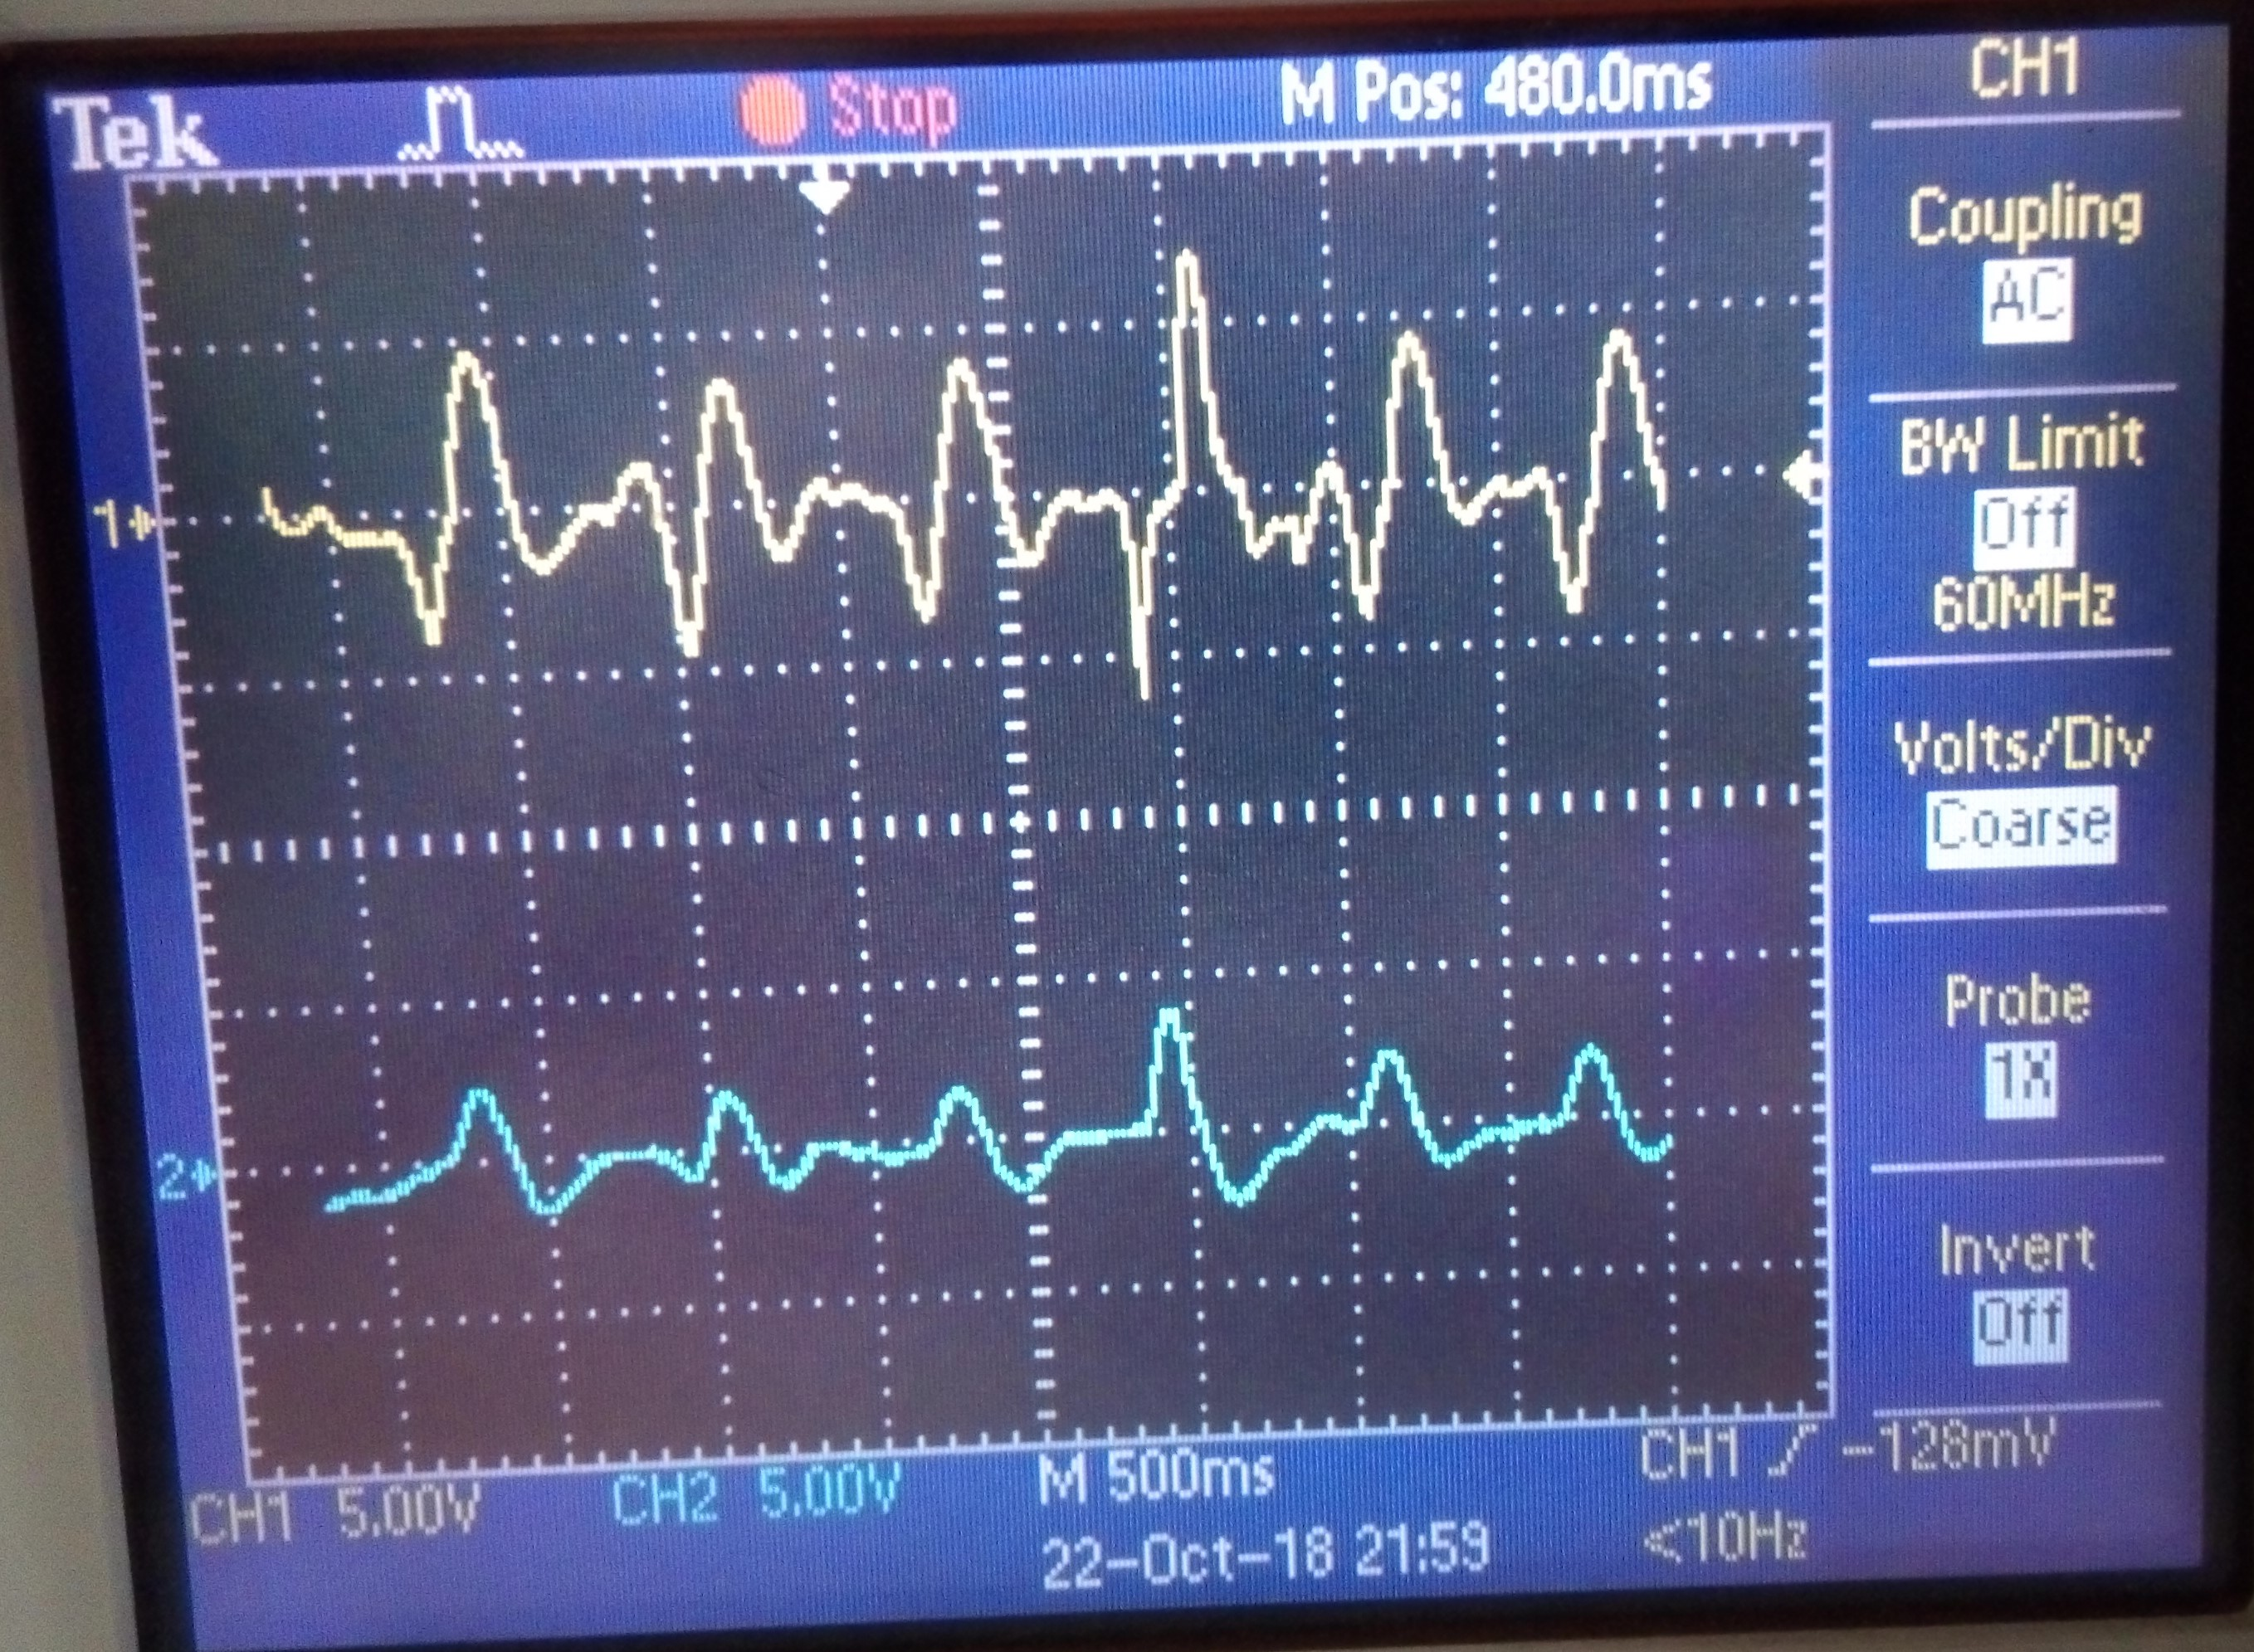
\includegraphics[width=0.65\textwidth]{Practica5/Images/etapa3_3.jpg}
            \end{figure}
            
        \textbf{Parámetros de medición (Vpp)}
            \begin{multicols}{2}
                \begin{itemize}
                    \item[\checkmark] \textbf{Amplitud máxima (Canal 1): 22 V}
                
                    \item[\checkmark] \textbf{Amplitud máxima (Canal 2): 13 V}
                    \item[\checkmark] \textbf{Base de tiempo: 500 ms}
            \columnbreak
                    \item[\checkmark] \textbf{Volts por división (CH1): 5 V}
                    \item[\checkmark] \textbf{Volts por división (CH2): 5 V}
                    \item[\checkmark] \textbf{Acoplamiento: Corriente Alterna}
                \end{itemize}
            \end{multicols}
            
            \textbf{Nota:} Si colocamos el dedo demasiado sueva, estamos permitiendo la entrada de ruido del exterior, obteniendo estos picos demasiado altos. Sin embargo, más adelante explicaremos por qué esto no afecta a la señal de salida final.
         
            \begin{figure}[h!]
                \centering
                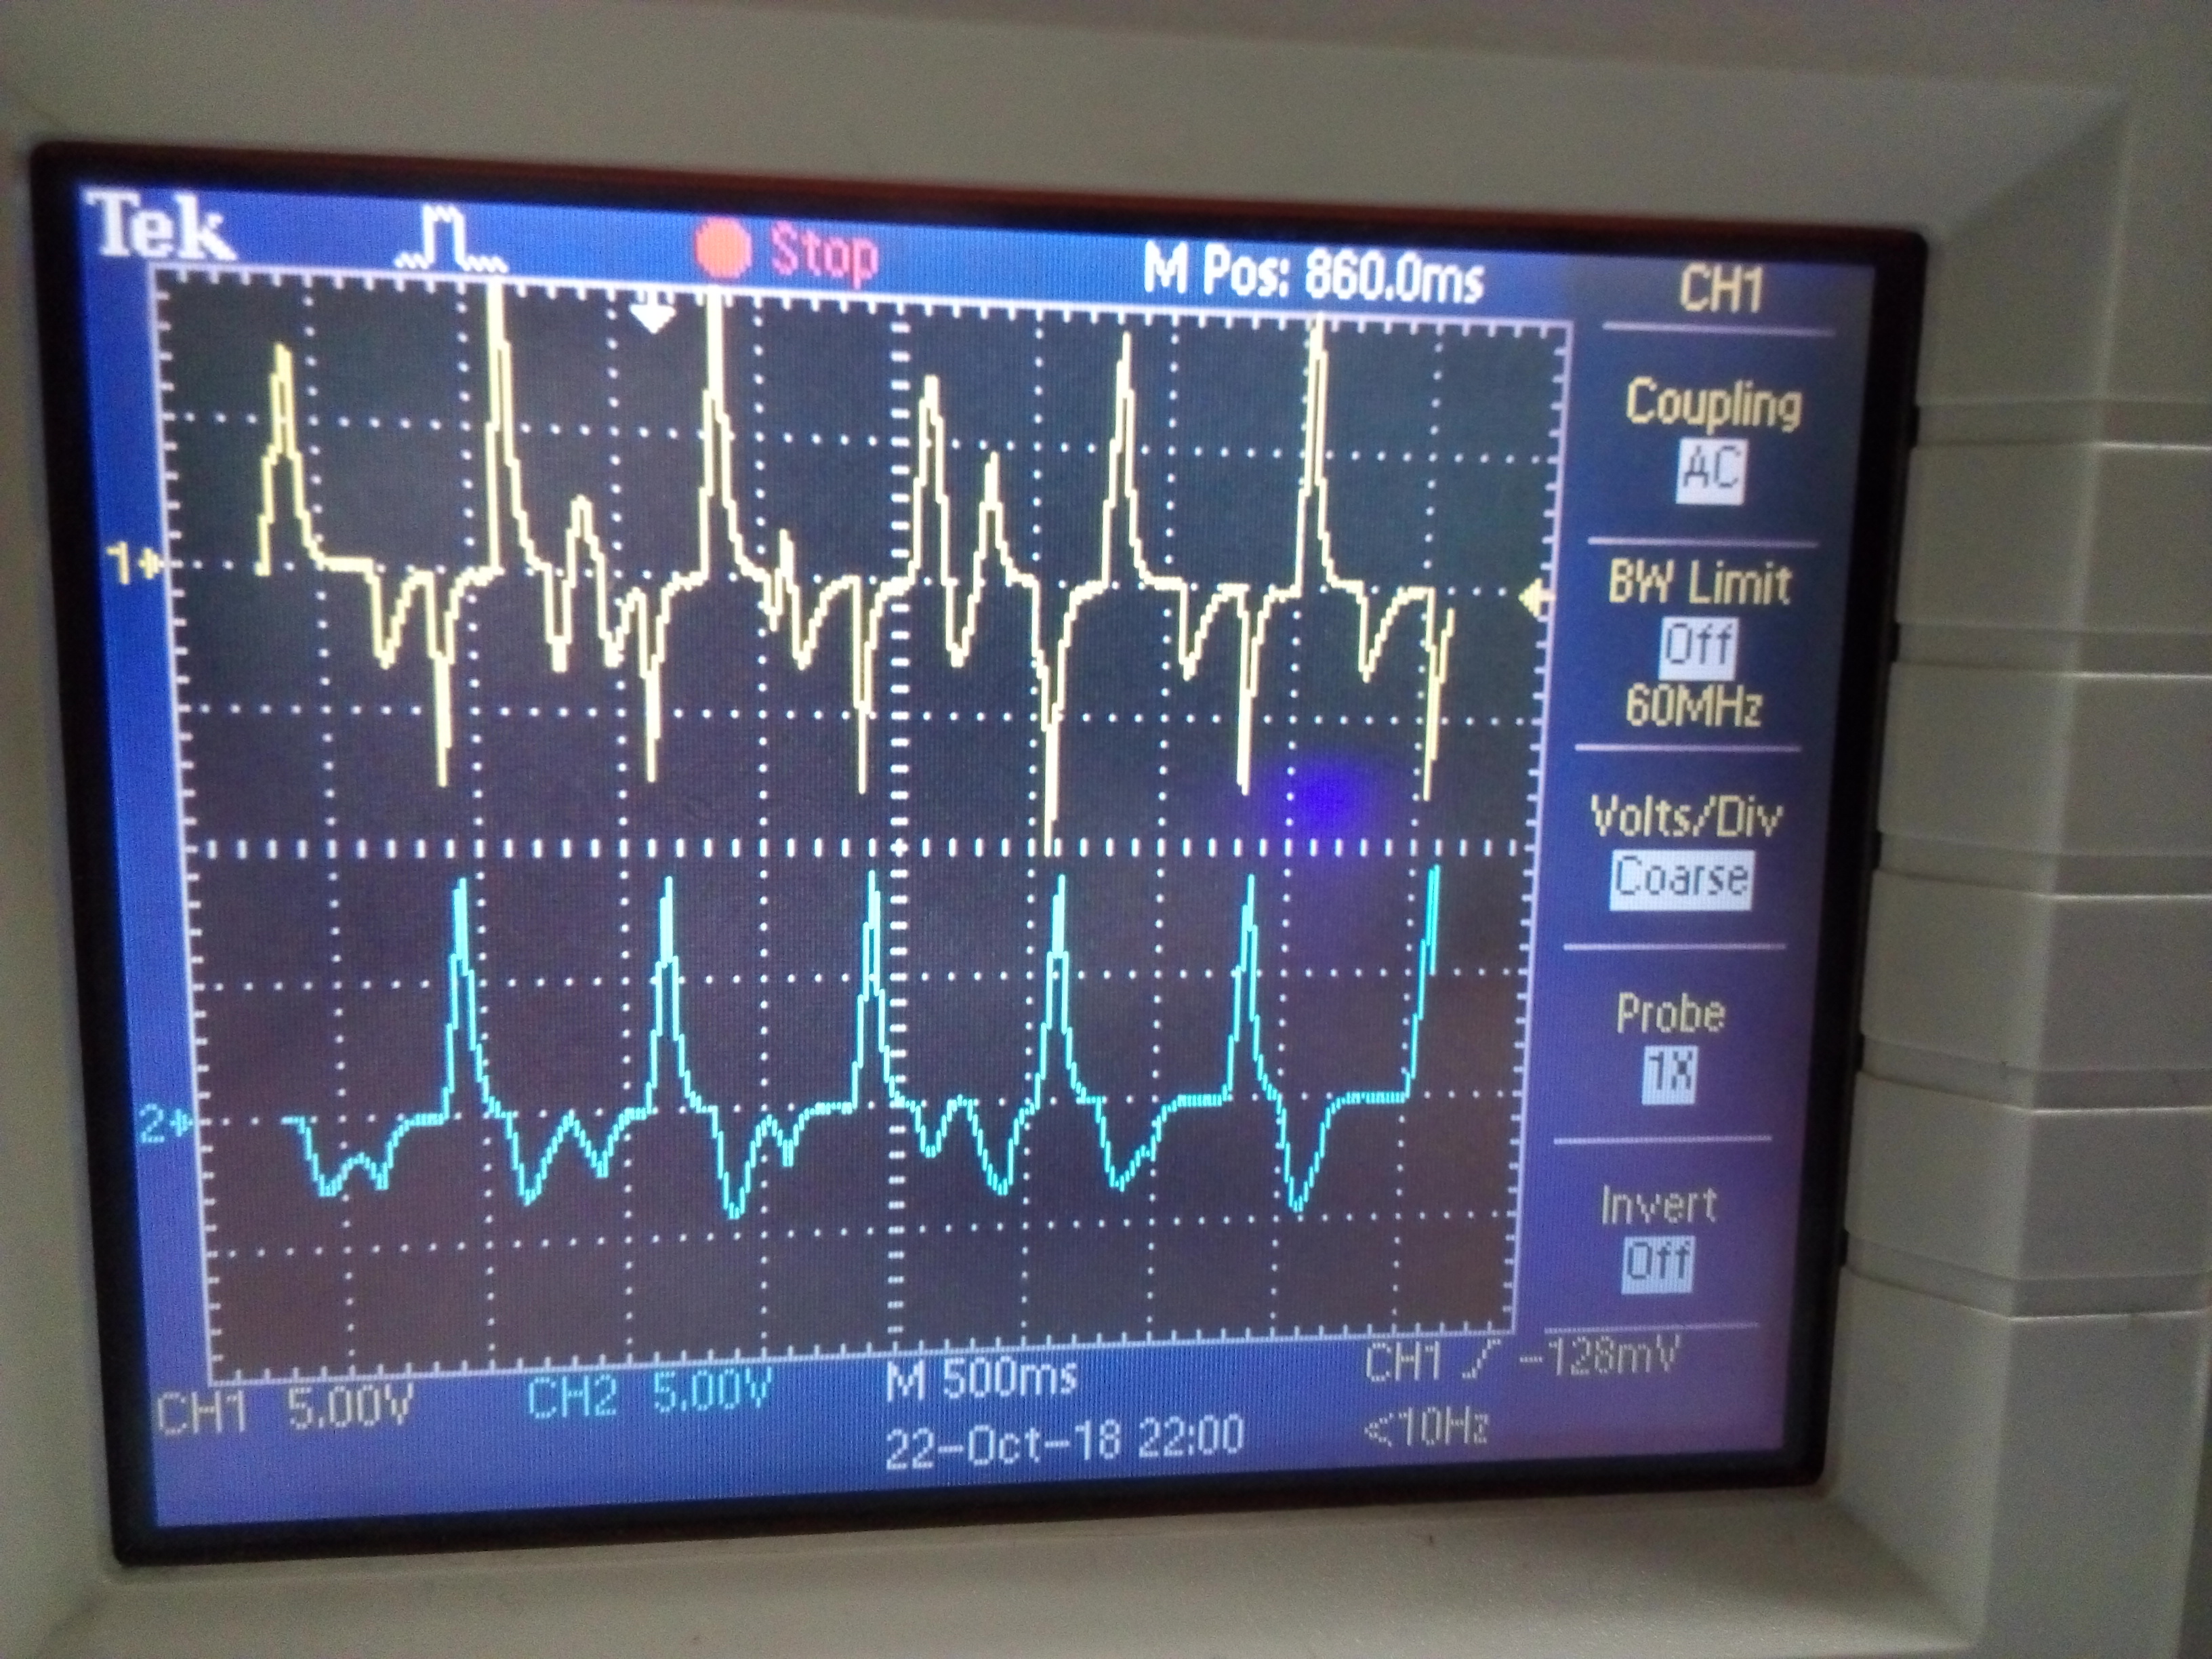
\includegraphics[width=0.65\textwidth]{Practica5/Images/etapa3.jpg}
            \end{figure}
        
        \newpage
        \subsection{PE 4 - Calibración (Diodo LED y Resistencia de Referencia)}
        \begin{multicols}{2}
            \subsubsection{Esquema}

                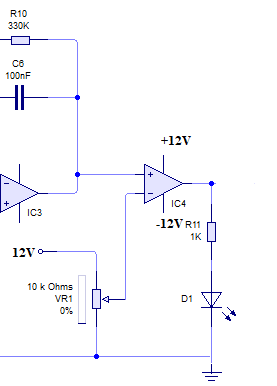
\includegraphics[width=0.35\textwidth]{Practica5/Images/pe4.png}

        \columnbreak
            \subsubsection{Circuito cableado}

                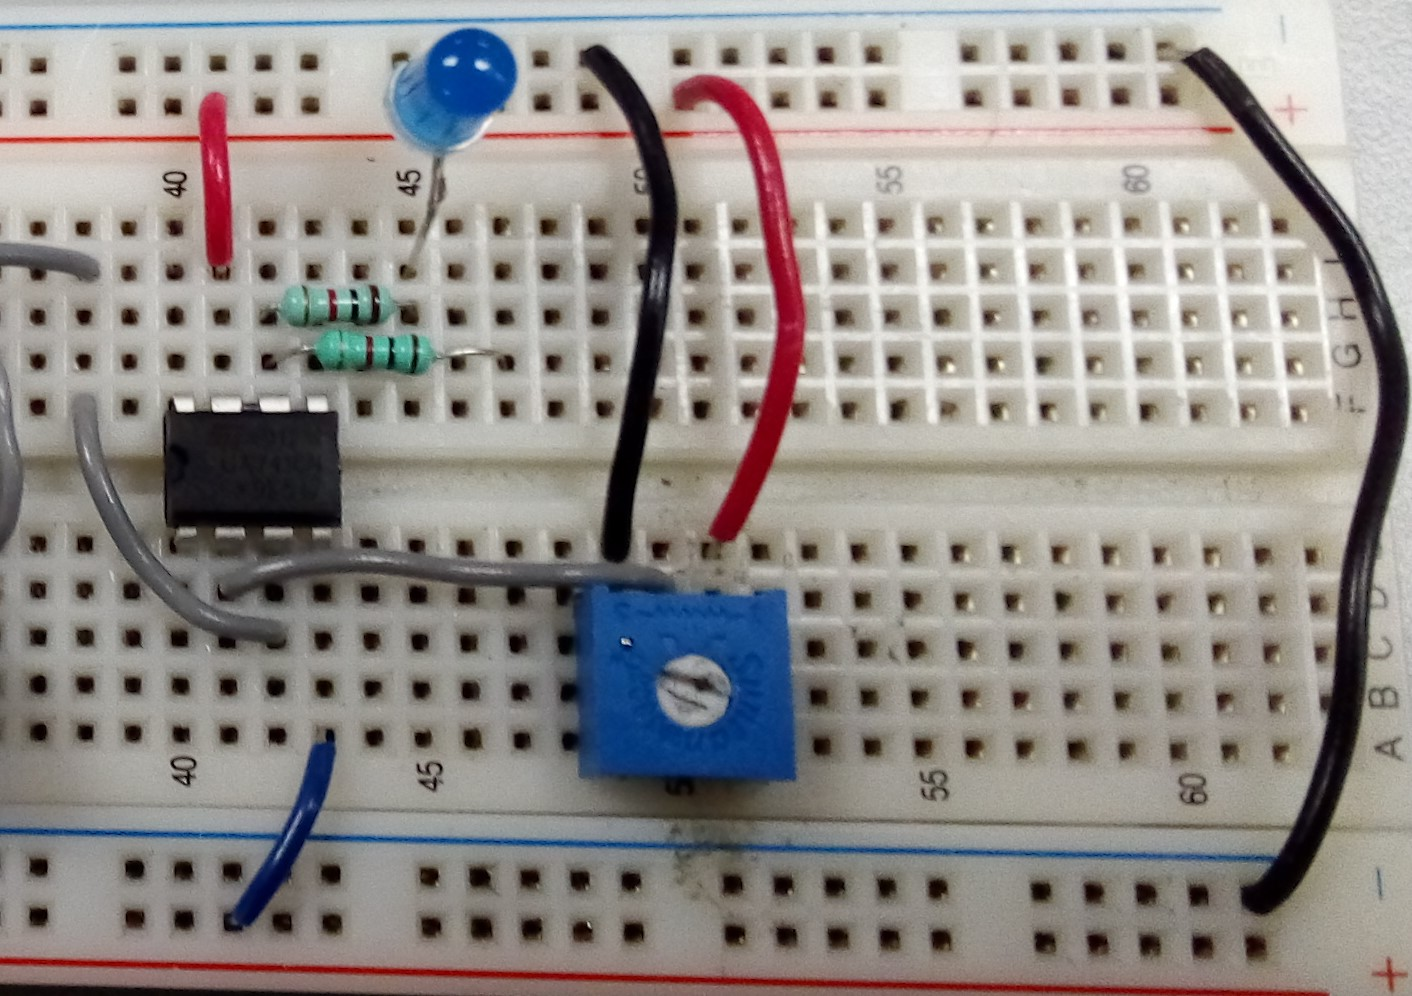
\includegraphics[width=0.5\textwidth]{Practica5/Images/cpe-4.jpg}

            \end{multicols}
            
            \subsubsection{Funcionamiento}
            En ésta etapa no realizaremos ningún tipo de acondicionamiento a la señal ya integrada, más bien la calibraremos.
            
            Con ayuda de un LM741 que posee una resistencia variable de referencia, un preset de 10 k$\Omega$, vamos a ir ajustando el circuito para que únicamente el LED encienda cuando existan picos los suficientemente grandes como para catalogarce como pulsos cardiacos.
            
            Recordemos que en etapas previas obteníamos picos medianos de voltaje que no rebasaban a aquellos de la amplitud máxima, pero a fin de cuentas entregaban un valor de voltaje cercano a los 5V (suficiente para encender un LED).
            
            Ajustando el preset, vamos ir discriminando éstos picos medianos de la señal que recibe el LED, para que solamente se ilumine con los picos de amplitud máxima, que corresponden a un pulso. 
            
            Es importante mencionar que en ésta etapa obtenemos también una señal cuadrada para hacer parpadear el LED cada vez que haya un pulso cardiaco.
            
            \textbf{Parámetros de medición (Vpp)}
            \begin{multicols}{2}
                \begin{itemize}
                    \item[\checkmark] \textbf{Amplitud máxima (Canal 1): 22 V}
                
                    \item[\checkmark] \textbf{Amplitud máxima (Canal 2): 30 V}
                    \item[\checkmark] \textbf{Base de tiempo: 500 ms}
            \columnbreak
                    \item[\checkmark] \textbf{Volts por división (CH1): 5 V}
                    \item[\checkmark] \textbf{Volts por división (CH2): 5 V}
                    \item[\checkmark] \textbf{Acoplamiento: Corriente Alterna}
                \end{itemize}
            \end{multicols}
            
            \textbf{Nota:} La linea amarilla (Canal 1) es la señal que sale del integrador (Canal 2) la que va hacia el LED.
         
            \begin{figure}[h!]
                \centering
                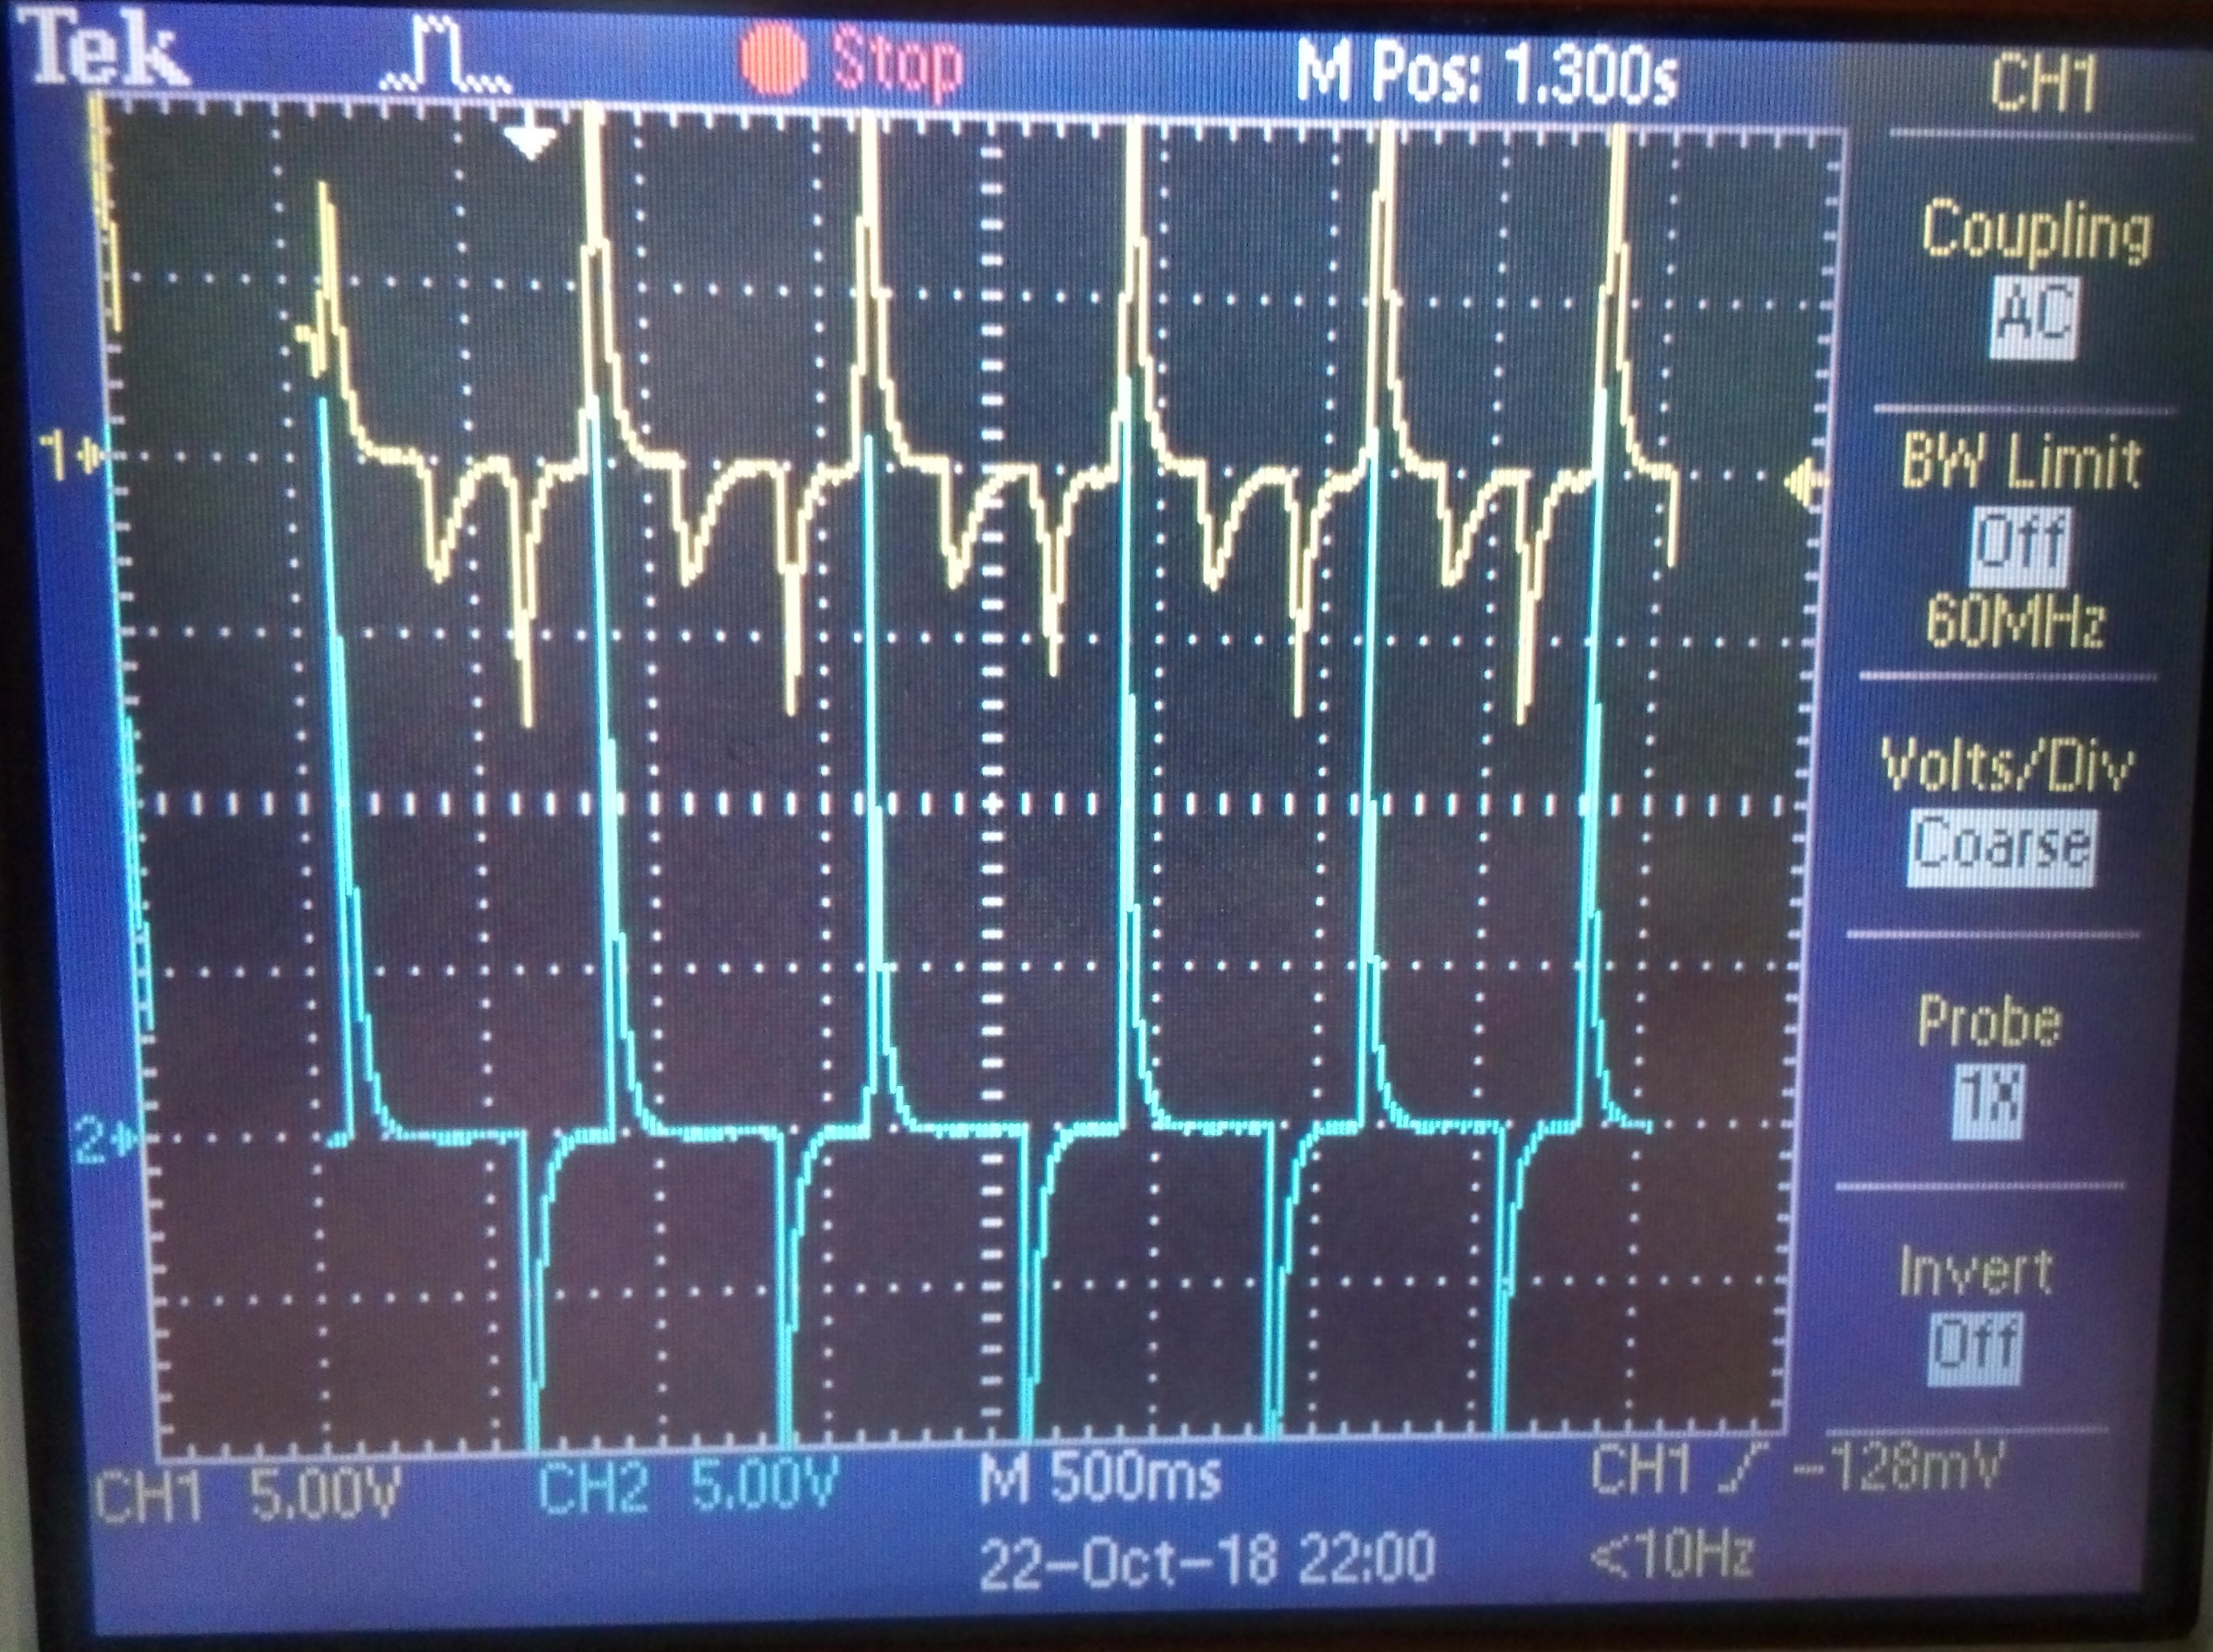
\includegraphics[width=0.65\textwidth]{Practica5/Images/etapa4_1ac.jpg}
            \end{figure}
            
            \newpage
            \textbf{Nota:} A nosotros nos interesa obtener la señal acoplada a Corriente Continua (señal cuadrada de 0 o 5 volts). Los parámetros de medición son los mismos que en la imagen anterior.
         
            \begin{figure}[h!]
                \centering
                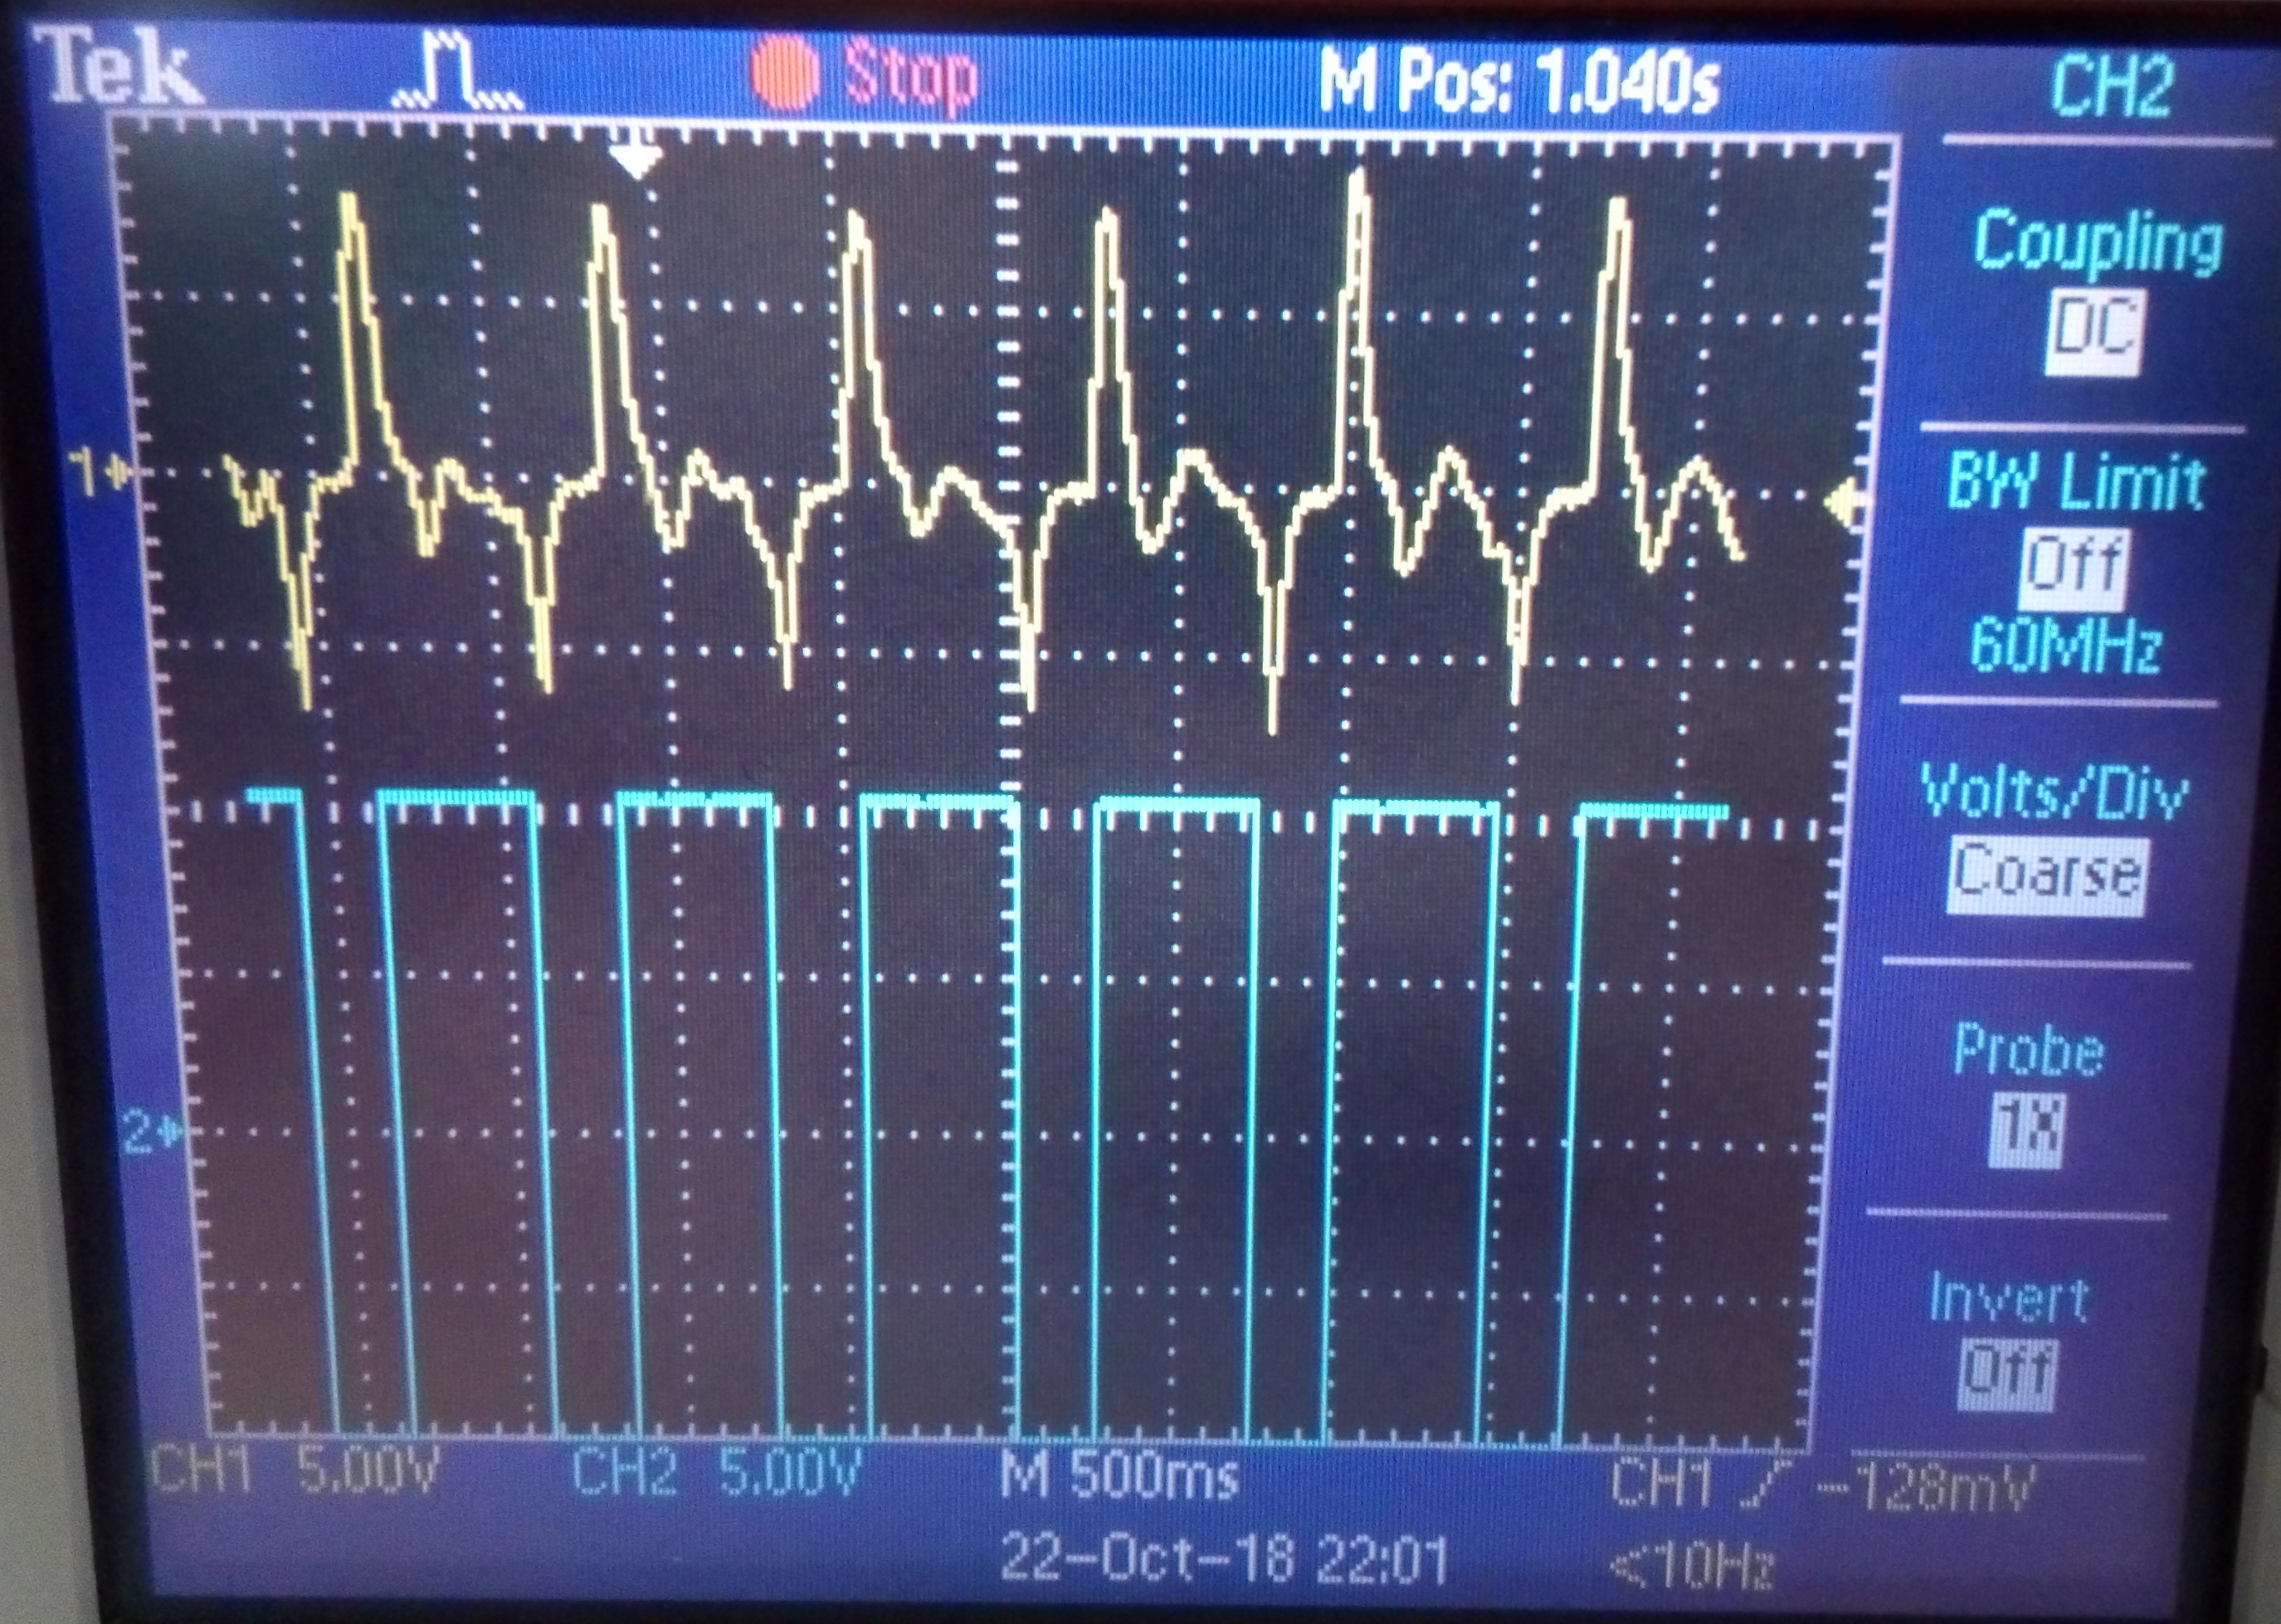
\includegraphics[width=0.65\textwidth]{Practica5/Images/etapa4dc.jpg}
            \end{figure}
            
            \subsection{Circuito completo}
            \subsubsection{Esquema}
            \begin{figure}[h!]
                \centering
                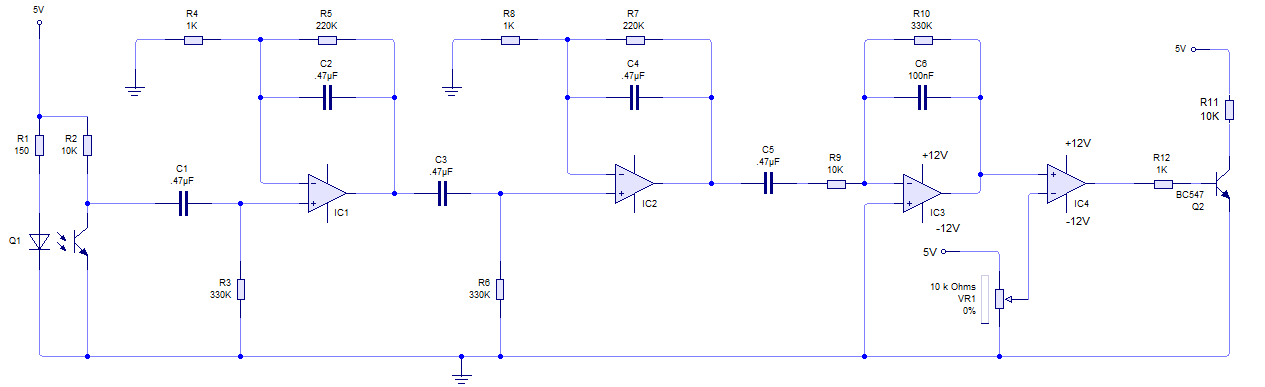
\includegraphics[width=1.1\textwidth]{Practica5/Images/circuito.png}
            \end{figure}
            
            \newpage
            \subsubsection{Circuito cableado}
            \begin{figure}[h!]
            \centering
                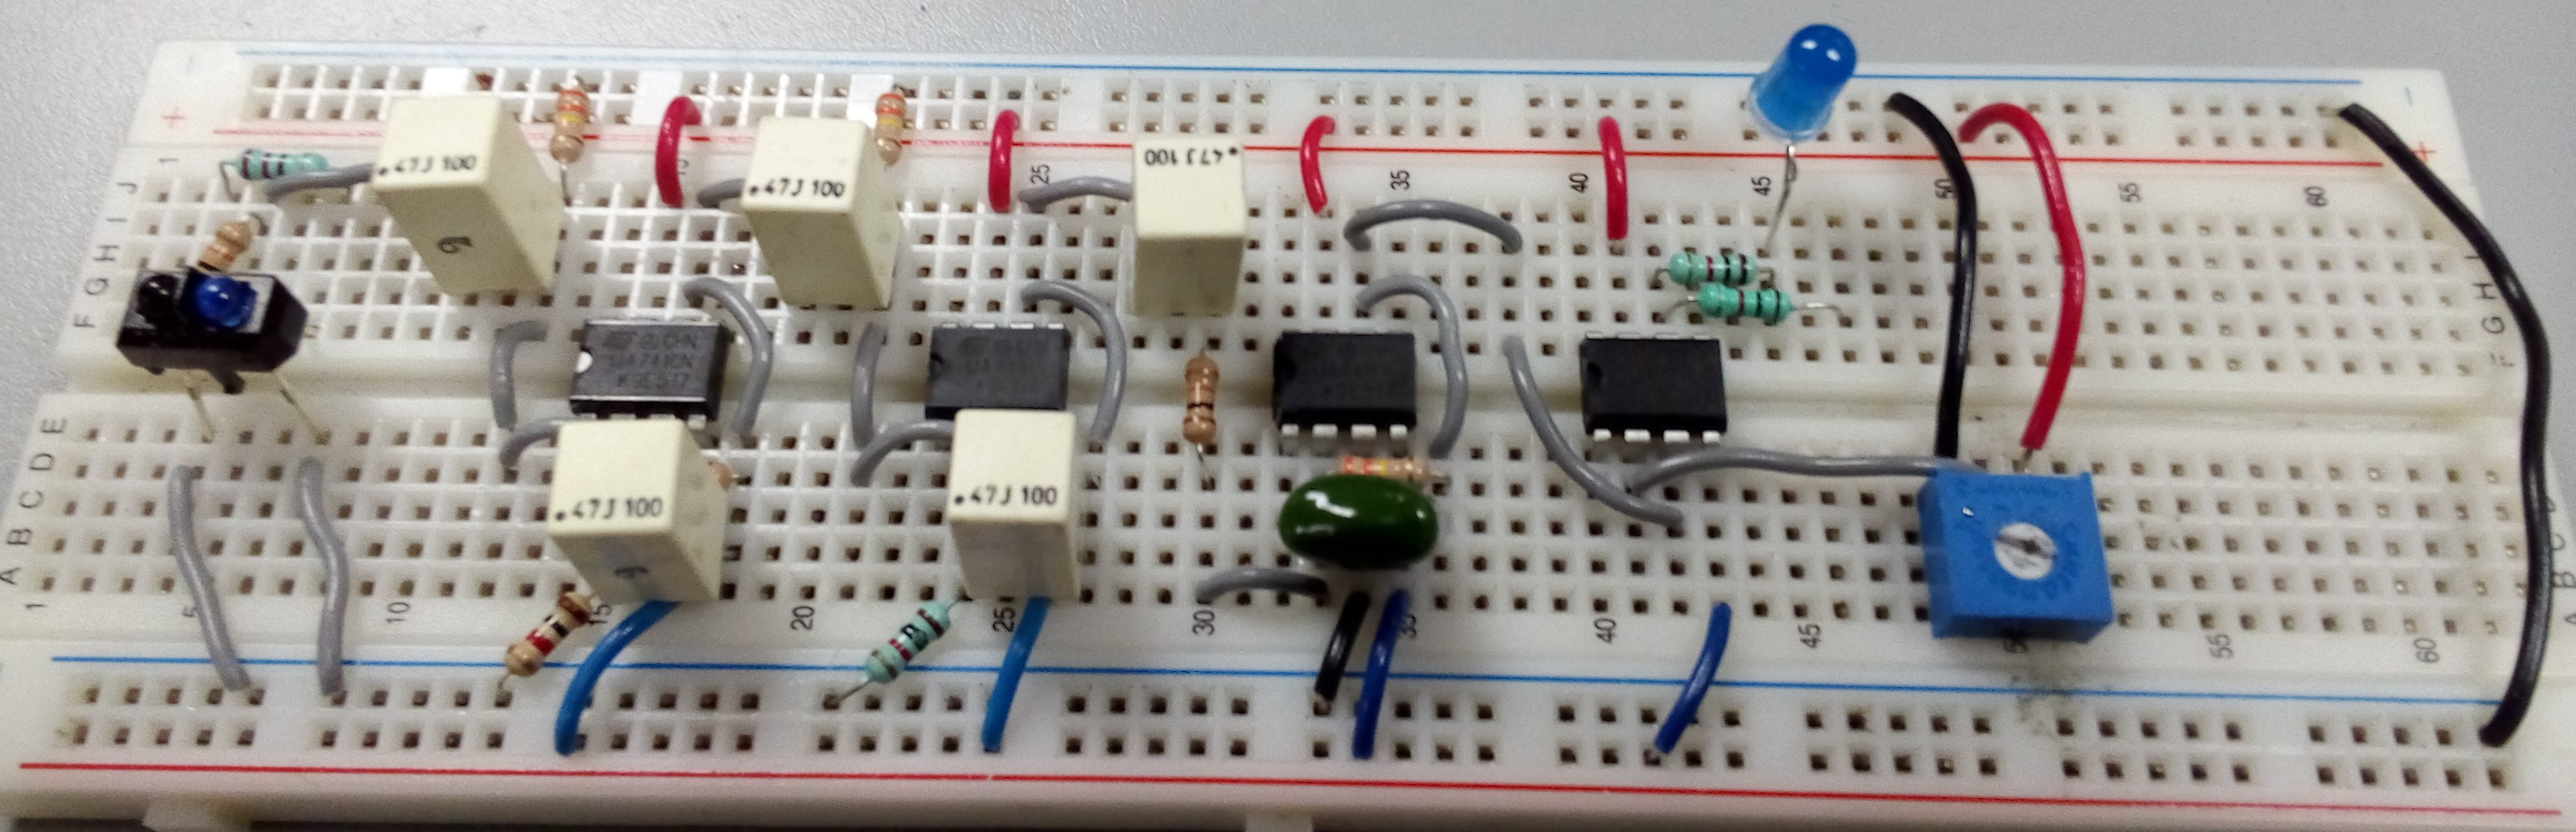
\includegraphics[width=\textwidth]{Practica5/Images/proto.jpg}
            \end{figure}
            
            \subsubsection{Funcionamiento completo}
            \begin{figure}[h!]
                \centering
                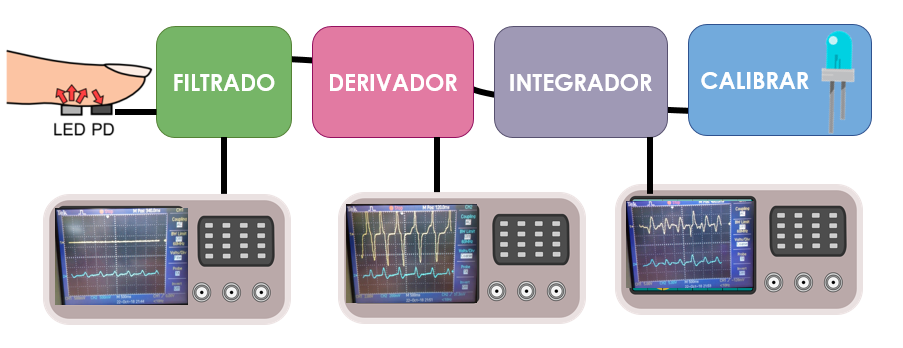
\includegraphics[width=\textwidth]{Practica5/Images/ETAPAS.PNG}
            \end{figure}

            \begin{itemize}
                \item Filtrado  \\
                Evita leer frecuencias extremadamente altas (ruido), proveniente de otras fuentes de luz y sombras.
                
                \item Derivador \\
                Hace que la salida sea proporcional a la velocidad de variación de la señal de la entrada.
                
                \item Integrador    \\
                Integra los picos pequeños a los grandes.
                
                \item Calibrar  \\
                Ajustan el circuito para que el LED encienda cuando existan picos los suficientemente grandes como para catalogarce como pulsos cardiacos reales.
            \end{itemize}

            \newpage
            \begin{figure}[h!]
               \centering
               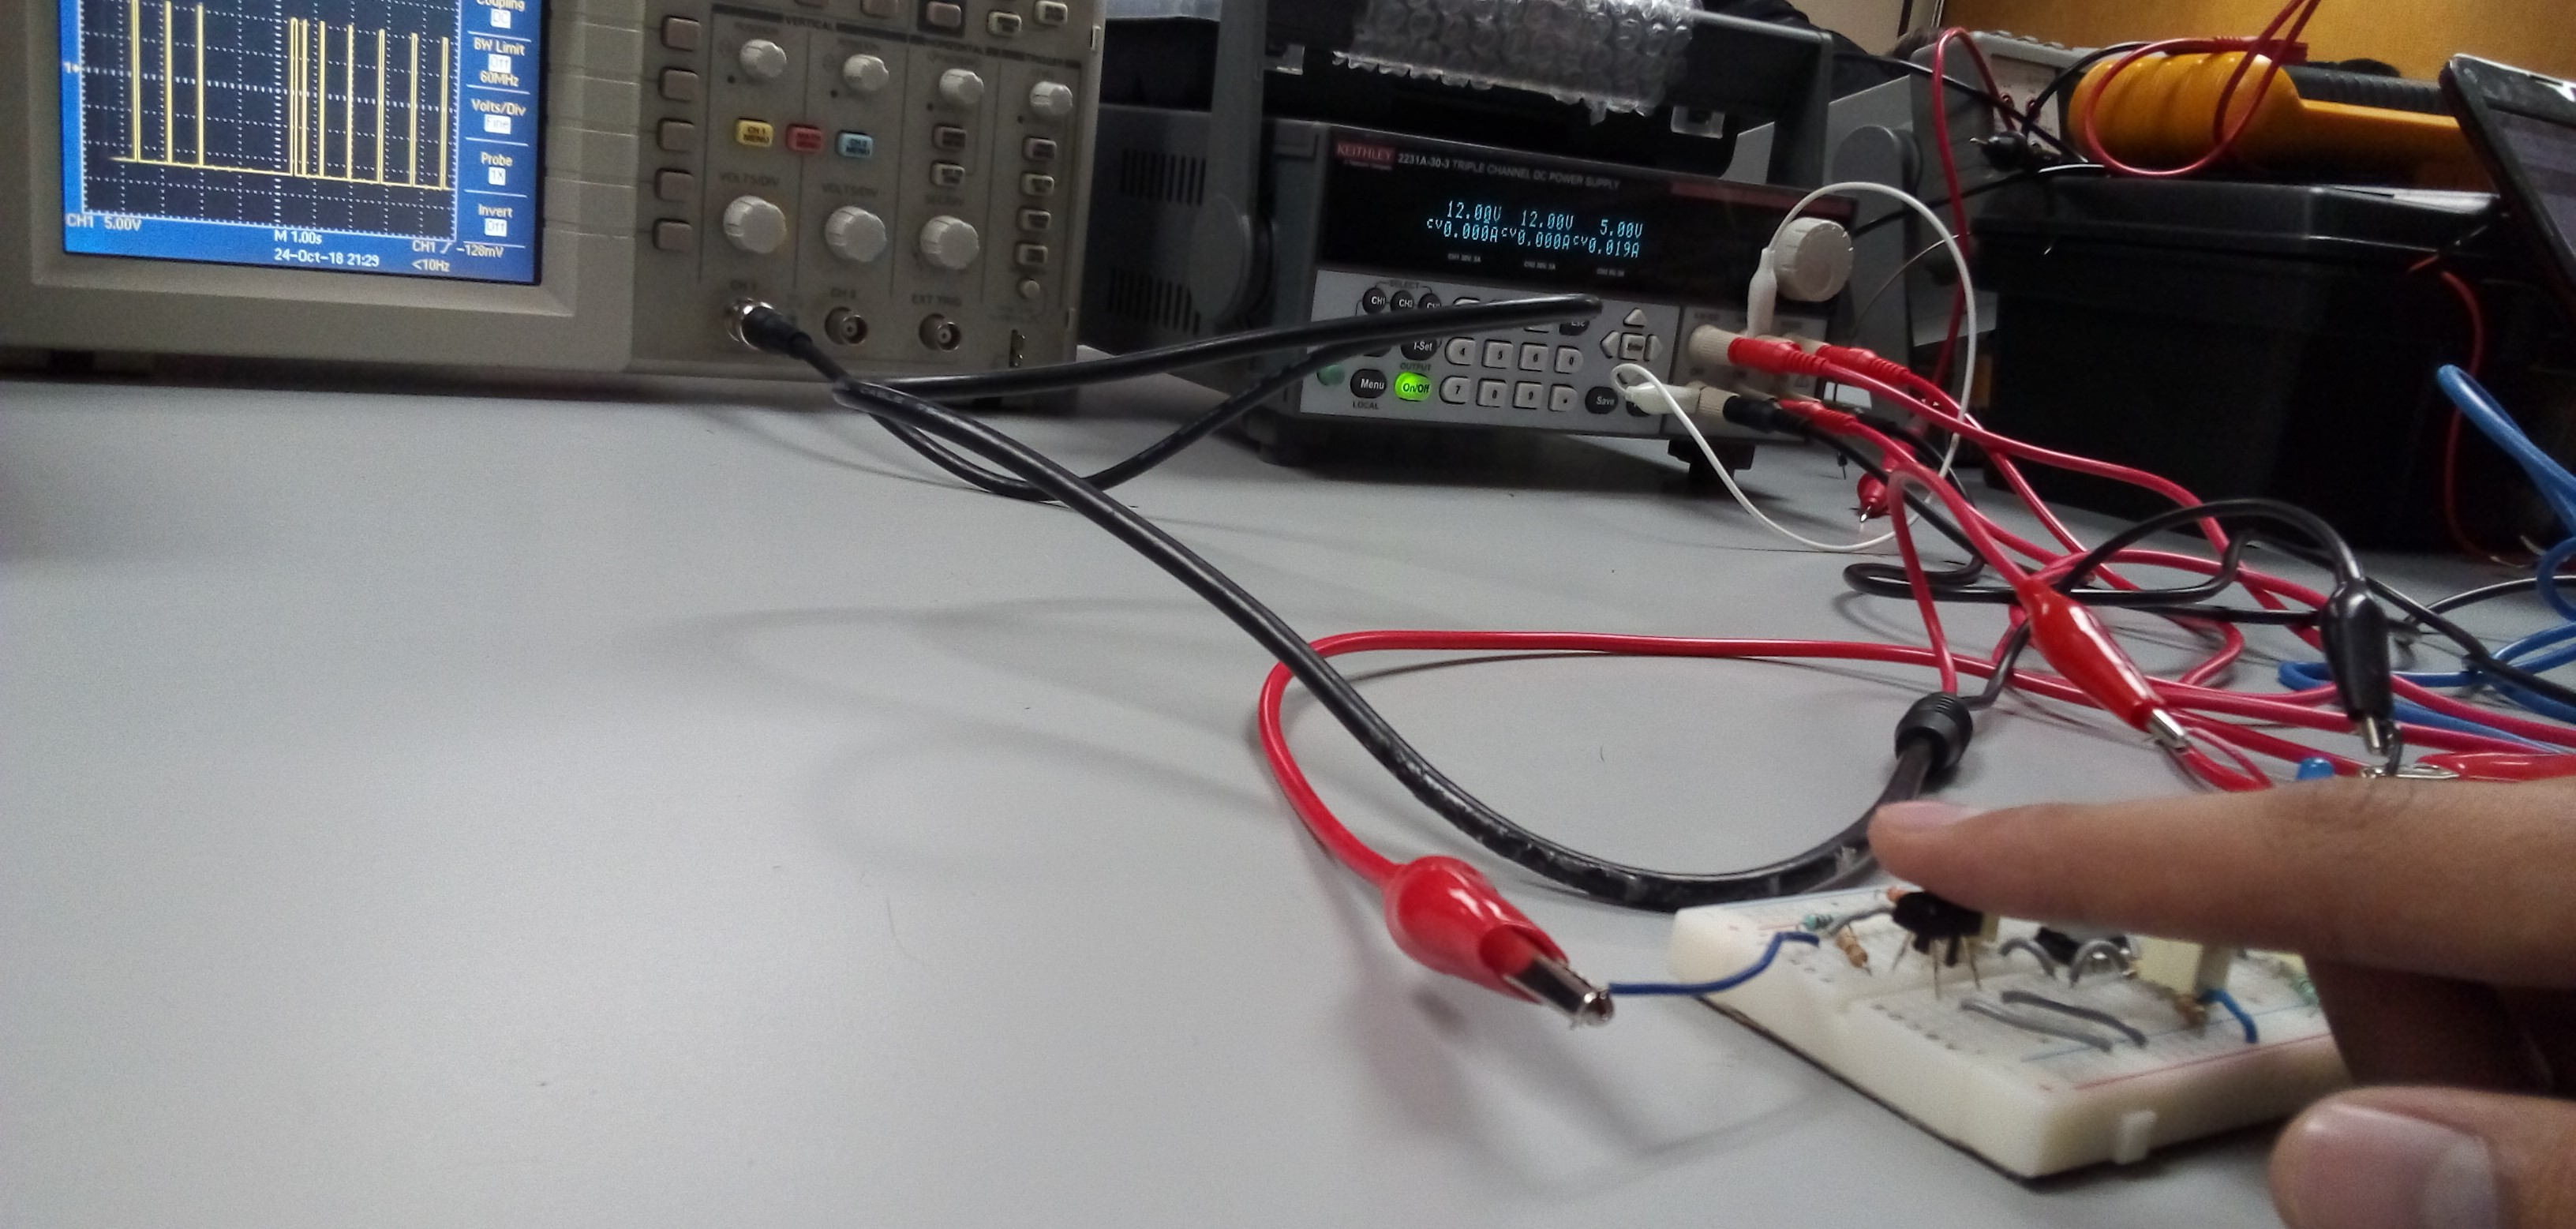
\includegraphics[width=0.75\textwidth]{Practica5/Images/fp3.jpg}
               
               \textbf{Lapso de tiempo entre pulsos.}
               
                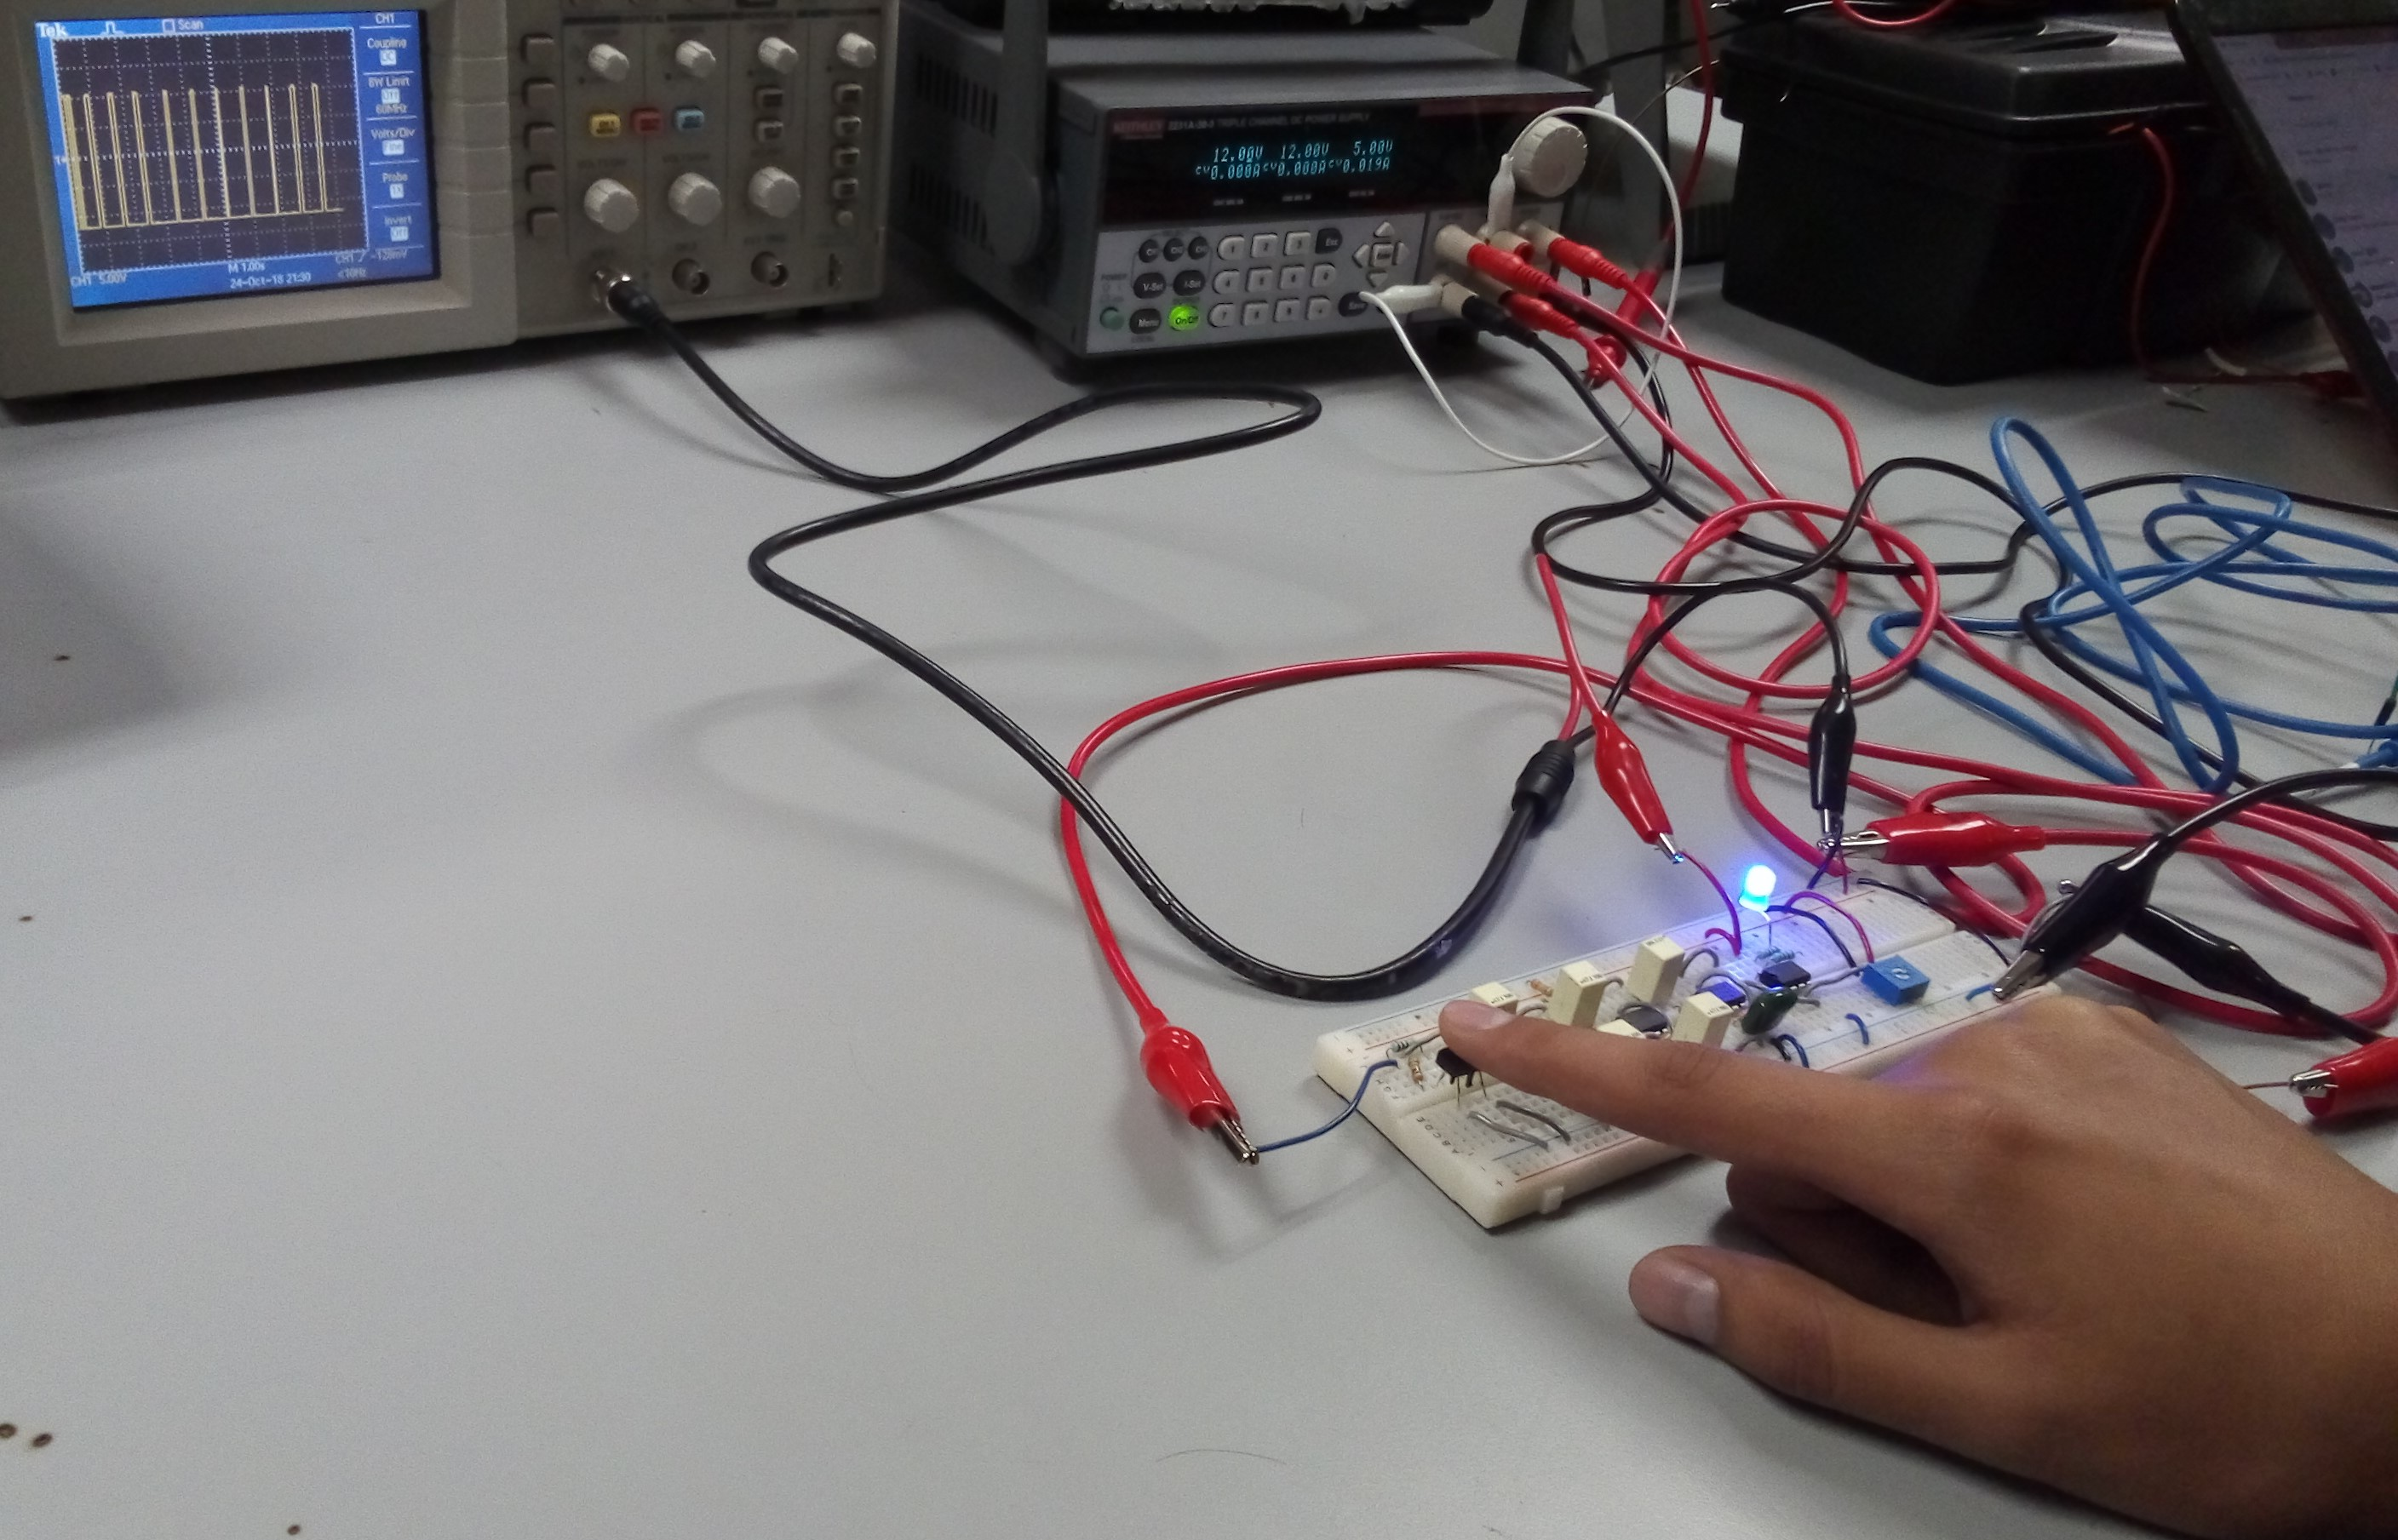
\includegraphics[width=0.75\textwidth]{Practica5/Images/fp2.jpg}
                
                \textbf{Aquí solamente medimos la señal que va hacia el diodo LED (Corriente Continua).}
                
                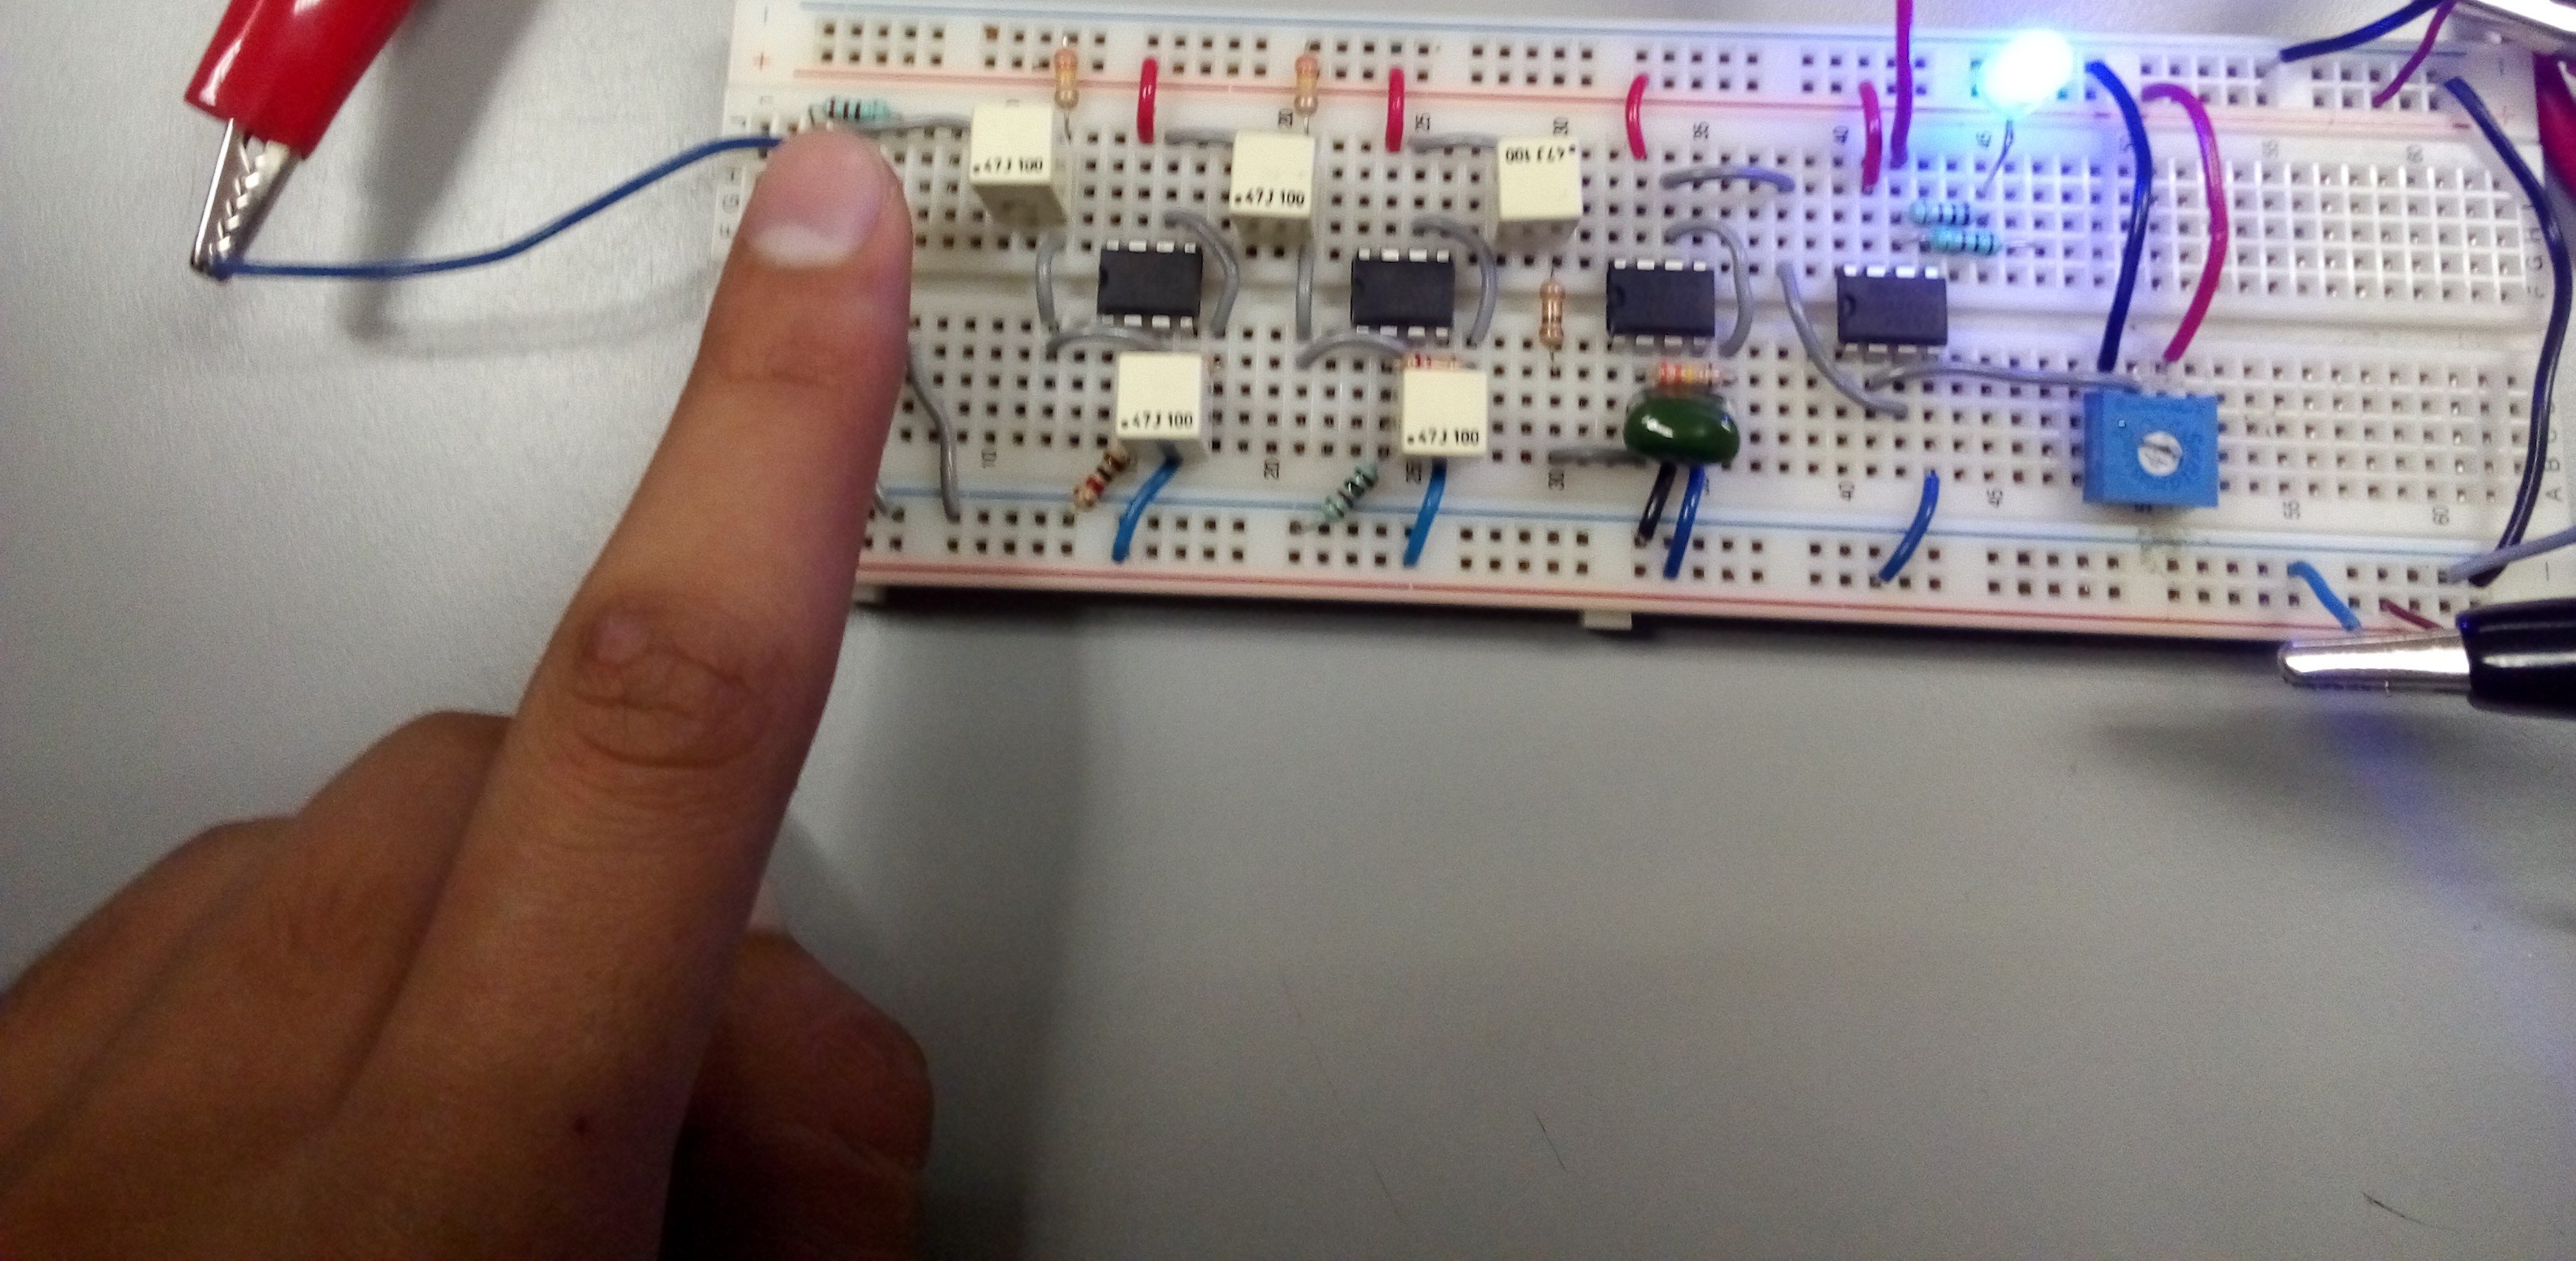
\includegraphics[width=0.75\textwidth]{Practica5/Images/fp1.jpg}
                
                \textbf{El LED se ilumina a cada pulso.}
                
                
           \end{figure}
           
    % /////////////////////////////////////////////////////////////////////
	%							OBSERVACIONES
	% ////////////////////////////////////////////////////////////////////
	\newpage
	\section{Observaciones}
	\begin{itemize}
            \item[\checkmark] El dedo debe colocarse de forma suave pero firme en el sensor TCRT5000L. 
            \item[\checkmark] Si se coloca de forma muy débil, obtendremos picos de voltaje sumamente altos, debido a la entrada de ruido entre nuestro dedo y el sensor.
            \item[\checkmark] Si se coloca de forma muy fuerte, obtendremos una señal muy débil y que a duras penas detecta los pulsos cardíacos.
            \item[\checkmark] El acoplamiento en Corriente Alterna en el osciloscopio lee una señal senoidal.
            \item[\checkmark] El acoplamiento en Corriente Continua en el osciloscopio lee una señal cuadrada. Ésta nos interesa para enviar la señal a un sistema digital, como la computadora o Arduino.
            \item[\checkmark] Con ayuda del preset, calibramos la señal que entrará al diodo LED, para así evitar que este encienda en picos lo suficientemente altos para este fin, pero que no corresponden a un pulso cardíaco real (cambios de luz y sombras).
            \item[\checkmark] El sensor TCRT5000L debe ser alimentado con un voltaje de 5V.
            \item[\checkmark] En los 3 vídeos anexados a este reporte se puede visualizar a mayor detalle el \\ comportamiento y funcionamiento del circuito. Link: \url{https://drive.google.com/drive/folders/1I-DoDsLIykFghbbf-bHl7X8hHt_w0T2P?usp=sharing}
            \item[\checkmark] La señal de salida posee una amplitud máxima sumamente alta, debido a la mala colocación del dedo en el circuito y una ganancia alta en la configuración de la última etapa de amplificación.
            \item[\checkmark] Con ayuda del preset ya mencionado anteriormente, también podemos reducir este exceso de voltaje a la salida.
    \end{itemize}
            
    

    % /////////////////////////////////////////////////////////////////////
    %                           CONCLUSIONES
    % ////////////////////////////////////////////////////////////////////
    \section{Conclusiones}
        \subsection{Aguilar Herrera Arianna Itzamina}
        Con esta práctica aprendimos a construir un fotopletismógrafo, el cual es un instrumento que nos ayuda a medir señales eléctricas, en el caso de esta práctica fueron las pulsaciones del corazón. 
        
        Para ello usamos el sensor de reflexión TCRT5000L, el cual fue el medio para introducir la señal al circuito que se construyó para darle un tratamiento en cada una de las etapas. 
        
        Primeramente al colocar el dedo de alguna persona se leyeron las pulsaciones, la señal que se leyó fue amplificada, para que pudiera ser notorio el cambio, además de filtrada, pues cuando no se colocaba el dedo generaba ruido, pero ese ruido no nos interesaba, por lo que era necesario discriminarlo, esto fue posible gracias a la ayuda del filtro, también fue necesario integrar la señal, después de haber sido amplificada y filtrada.
        
        Por último fue necesario hacer ajustes, ya que como hemos visto en prácticas anteriores, y el cual es un objetivo de la materia, hay que saber retroalimentar el circuito, es decir, después de hacerlo, mejorarlo, corrigiendo fallas que pueda tener, una de las fallas más notorias fue una falla en las resistencias, aunque ese fue más error que algo por mejorar, un ejemplo de algo por mejorar es el ruido que mostraba el instrumento antes de colocar el dedo, pues el osciloscopio mostraba una señal la cual era producida por el ruido en el ambiente, pero eso lo pudimos corregir gracias al preset colocado al final del circuito. 
        Como vemos, se lograron los objetivos de la práctica, y propiamente de la materia, al introducir la etapa de retroalimentación a este instrumento. 
        
        La elaboración de esta práctica nos enseñó otro uso que le podemos dar a la electrónica en un ambiente médico. 
        
      
        \subsection{Nicolás Sayago Abigail}
            Al finalizar la práctica se hizo un instrumento  fotopletismógrafo, con el cuál podemos medir los pulsos cardíacos, utilizando el sensor de reflexión infrarrojo TCRT5000L.
            
            A lo largo de la practica pudimos interpretar y leer las señales que se generaban por el pulso cardíaco  en cada una de las diferentes etapas.
            
            Algo que personalmente pude notar, fue la importancia de usar las resistencias correctas debido a que al cablear, no puse las resistencias debidas y eso provoco que nuestra señal no saliera bien amplificada.
            
            Es importante notar también que en esta ocasión usamos un amplificador operacional derivador que nos ayudo cuando veíamos señales cuadradas y triangulares en el caso de los picos, con el amplificador operacional integrador pudimos ver los picos grandes y pequeños.
            
            Finalmente, puedo resumir que cada vez es más interesante hacer un instrumento con costos bajos y circuitos fáciles de armar.
            
        \subsection{Ramos Diaz Enrique}
        Trabajar con señales provocadas por los pulsos cardíacos del corazón es una forma muy interesante de estudiar y repasar conceptos de la electrónica analógica, la digital y la instrumentación.
        
        Utilizando sensores reflectivos, logramos leer la señal producida por un pulso del corazón en un dedo de la mano, midiendo la cantidad de luz que pasa a través del flujo sanguíneo de este.
        
        Como se ha venido trabajando, es necesario acondicionar este señal, pues es imposible de manejar e interpretar si la tomamos directamente de la salida del sensor que además es del orden de los mili volts.
        
        En primera instancia, se filtra para eliminar el ruido que se cuela por el sensor, y de paso amplificar ligeramente la señal. Luego, la pasamos por un amplificador operacional derivador para detectar los cambios del pulso cardíaco, pues existen picos de voltaje medios, que más adelante los integraremos a los picos de voltaje máximos, por medio de un amplificador operacional integrador, que representarán cada pulso.
        
        Finalmente, ya acondicionada, simplemente la calibramos por medio de una resistencia de referencia para que un diodo LED detecte únicamente aquellos picos con amplitud máxima, ya que existen picos que llegan a alcanzar un voltaje necesario para iluminar el LED, pero que no corresponden realmente a un pulso.
        
        Ésta es una práctica muy didáctica que nos ayuda a comprender conceptos básicos de la electrónica en general, y llamar nuestra atención hacía ella.
        
      
        \newpage
    %/////////////////////////////////////////////////////////////////
    %                           ANEXOS
    %/////////////////////////////////////////////////////////////////
    
    \section{Anexos}
    \subsection{LM741}
	        \begin{figure}[h!]
                \centering
                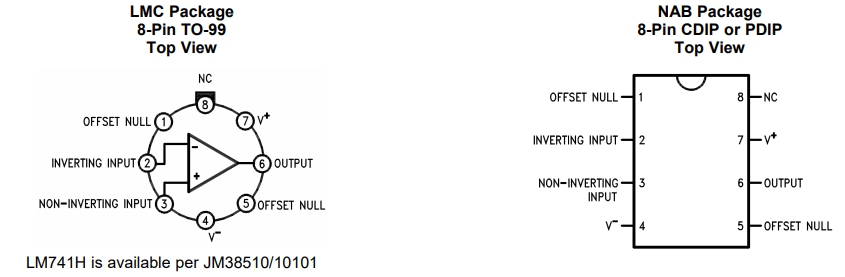
\includegraphics[width=\textwidth]{Practica4/Images/lm741.PNG}
            \end{figure} 
	        El amplificador operacional LM741 debe estar alimentados por una fuente de +12 V y -12 V en serie. [Consultar hoja de especificaciones del LM741].
	        
	        \begin{figure}[h!]
                \centering
                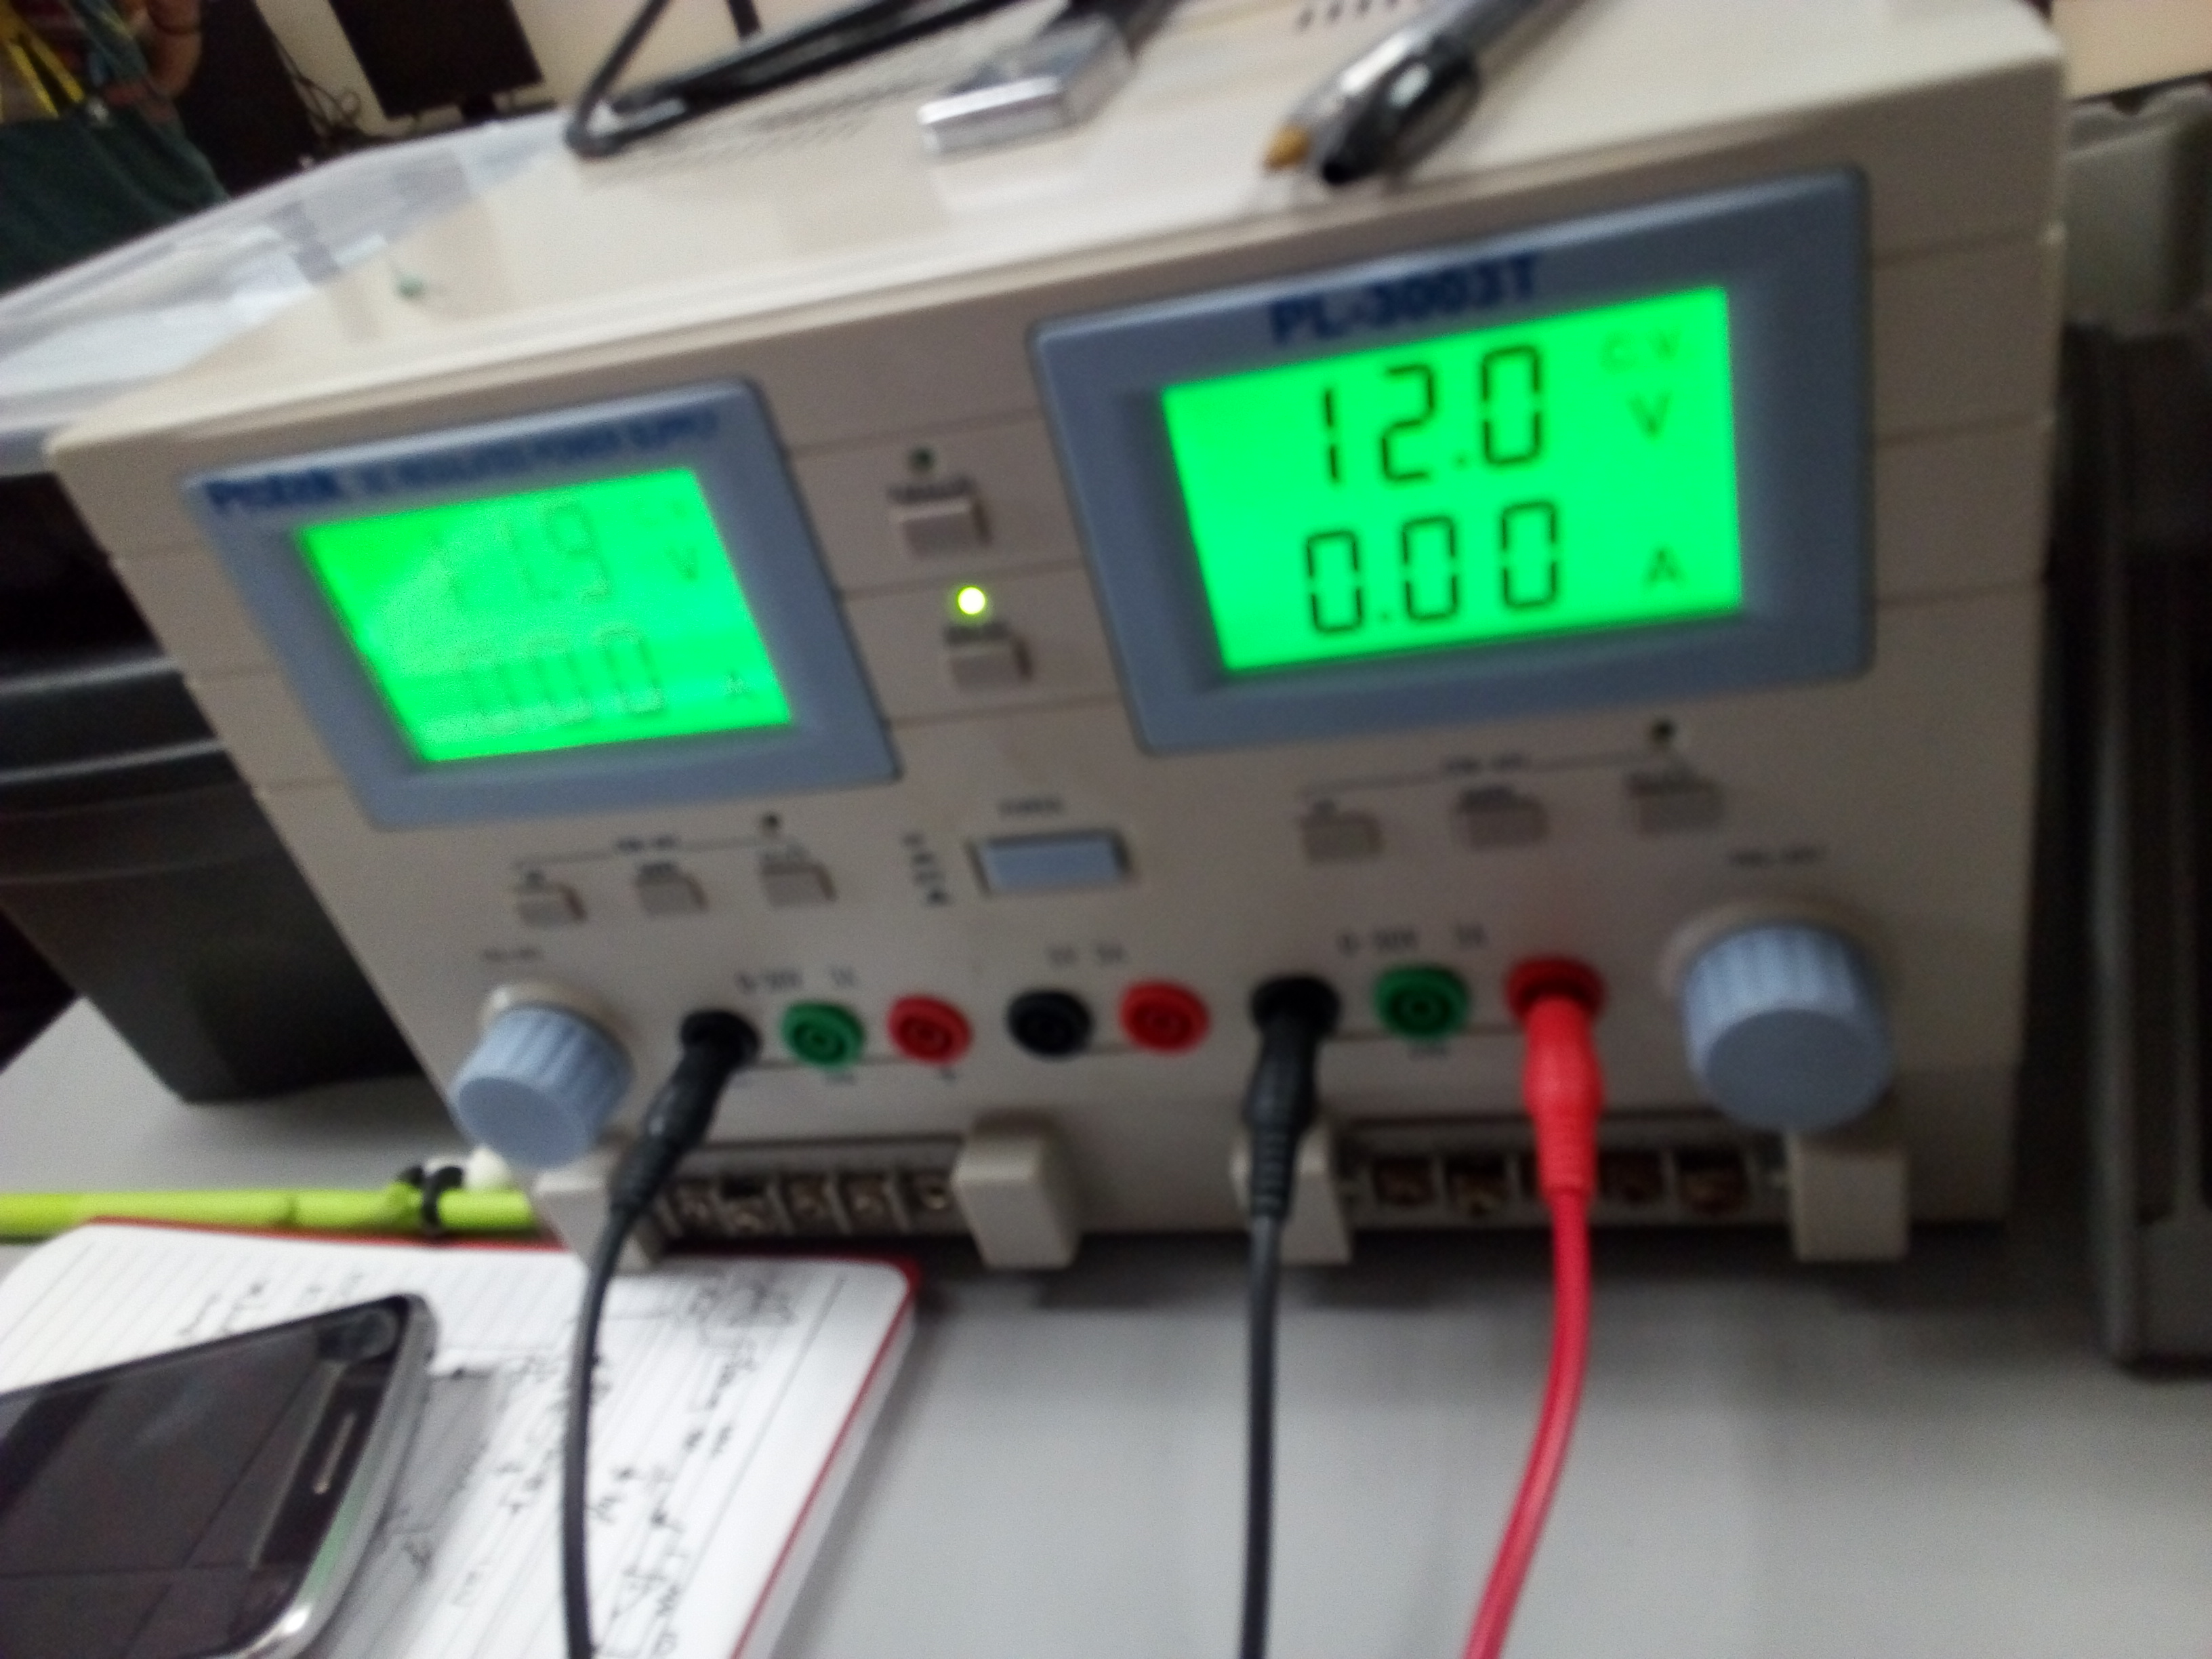
\includegraphics[width=0.7\textwidth]{Sismografo/Images/fuente.jpg}
            \end{figure} 
        \newpage
    \subsection{Sensor TCRT5000L}
    
    
    El TCRT5000 y TCRT5000L son sensores reflectivos que incluyen un emisor de infrarrojos y un fototransistor en un paquete de plomo que bloquea la luz visible. El paquete incluye dos clips de montaje. TCRT5000L es la versión de plomo más larga. Debe alimentarse con 5 V.
    
    \begin{figure}[h!]
                \centering
                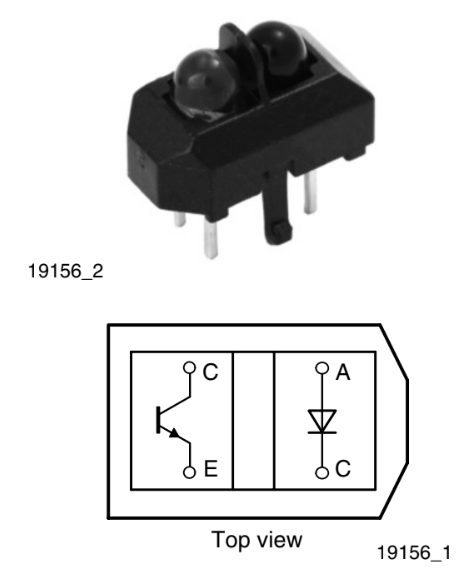
\includegraphics[width=0.5\textwidth]{Practica5/Images/tcrt.PNG}
            \end{figure} 
    
       

    %/////////////////////////////////////////////////////////////////
    %                           REFERENCIAS
    %/////////////////////////////////////////////////////////////////

    \nocite{ref1, ref2, ref3, ref4}
    \bibliography{ref5}
        

    \end{document}
